\documentclass[a4paper, 12pt]{article}
\usepackage{graphicx}
\usepackage[margin=1in]{geometry}
\usepackage{titlesec}
\usepackage{indentfirst}
\usepackage{setspace}
\usepackage{amsmath}
\usepackage{amssymb}
\usepackage[outputdir = ../]{minted}
\usepackage[svgnames]{xcolor}
\usepackage[hidelinks]{hyperref}
\usepackage{tabularray}
\usepackage{graphbox}
\usepackage{float}
\usepackage{comment}
\usepackage{mathrsfs}
\usepackage{multirow}
\usepackage[
    backend=biber,
    style=authoryear,
  ]{biblatex}
\addbibresource{bib.bib}

\titleformat{\section}[block]{\large\bfseries}{\thesection}{0.5cm}{}
\titleformat{\subsection}[block]{\normalfont\bfseries}{\thesubsection}{0.5cm}{}
\titlespacing{\subsection}{8pt}{8pt}{8pt}

\newcommand\mefvm{%
    \textit{m}\kern-.1em%
    \raise0.5ex\hbox{\textit{e}}\kern-.1em%
    \textit{f}\kern-.2em%
    \raise-0.5ex\hbox{\textit{v}}\kern-.05em%
    \textit{m}
}
\renewcommand{\labelitemi}{-}
\renewcommand{\labelitemii}{-}

\begin{document}
\doublespacing
\begin{titlepage}
    \begin{center}
        
\includegraphics[width=0.8\textwidth]{HW4/university1.pdf}\\
        
        \textbf{ME485: Computational Fluid Dynamics \\ Using Finite Volume Method}

        \vspace{0.5cm}
        Homework 4
            
        \vspace{1.5cm}

        \textbf{Uğur Ozan Baygeldi}\\
        \textbf{Ali Kaya}\\ 
        \textbf{Onur Kakilli}\\~\\
        Group 15
        
    \end{center}
\end{titlepage}
\section{Introduction}
This homework is different from the first three as there is no need to implement any code. (\cite{hw3}) Instead, this homework requires an analysis of the methods implemented to \mefvm\hspace{-0.3em}, asking for a comparison of the different convection flux computation methods implemented under different initial conditions, boundary conditions, and using different time discretization methods.
\section{Roadmap}
As there is no need to implement any code, there is no \verb|system.py| to give guidance. Thankfully, the homework document provides sufficient direction. (\cite{lect}) The report will cover the following, with text in brackets indicating the implemented name within \mefvm:
\begin{itemize}
    \item Explanation of the Convection Flux Computation Methods
    \begin{itemize}
        \item Roe [\verb|roe|]
        \item RoeM [\verb|roem|]
        \item Rotated-RoeM [\verb|rotated-roem|]
        \item AUSMPW+ [\verb|ausmpw+|]
        \item AUSM$^+$-up [\verb|ausm+up|]
        \item HLLEM [\verb|hllem|]
        \item Rusanov [\verb|rusanov|]
    \end{itemize}
    \item Explanation of the Benchmark Problems
    \begin{itemize}
        \item Double Mach Reflection (Canceled)
        \item Forward Facing Step
        \item Flow Over a Circular Bump
        \item Scramjet Inlet Flow Model with Different Boundary Conditions [\verb|slip-wall|, \verb|sup-in|, \verb|sub-outp|, \verb|far|]
    \end{itemize}
\end{itemize} \par
Essentially this report covers a variety of topics commonly encountered in the CFD world.
\section{Explanation of the Convection Flux Computation Methods}
In this chapter, the convective flux computation methods utilized in this report will be summarized. 
\subsection{Roe [\texttt{roe}]}\label{roe}
Roe method attempts to find a Jacobian matrix $A = \partial\textbf{F}/\partial\textbf{u}$ such that:
\begin{equation}
    \begin{split}
        \textbf{u}_t+\textbf{F}_x&=0 \\
        \textbf{u}(x,0)&=\textbf{u}_0(x)
    \end{split}
\end{equation} \par
This $A$ matrix is then approximated as $\tilde A$, a constant matrix, that satisfies the follow the following conditions (\cite{roe}):
\begin{itemize}
    \item Constitutes a linear mapping from the vector space \textbf{u} to the vector space \textbf{F}
    \item As $\textbf{u}_L \rightarrow{} \textbf{u}_R \rightarrow{} \textbf{u}$, $\tilde A(\textbf{u}_L,\textbf{u}_R) \rightarrow{} A(\textbf{u})$
    \item $\forall\:\textbf{u}_L, \textbf{u}_R$, $\tilde A(\textbf{u}_L,\textbf{u}_R)\times(\textbf{u}_L- \textbf{u}_R)=\textbf{F}_L-\textbf{F}_R$
    \item Eigenvectors of $\tilde A$ are linearly independent.
\end{itemize} \par
To meet the criteria, Roe follows the following path (\cite{roe}):
\begin{equation}
    \textbf{u}(\theta)=\textbf{u}_L+\theta(\textbf{u}_R-\textbf{u}_L),\:\: d\textbf{u}=(\textbf{u}_R-\textbf{u}_L)d\theta
\end{equation}
\begin{equation}
    \textbf{F}(\textbf{u}_R)-\textbf{F}(\textbf{u}_L)=\int^1_0A(\theta)d\theta\cdot(\textbf{u}_R-\textbf{u}_L) \rightarrow{} \tilde A=\int^1_0A(\theta)d\theta\
\end{equation} \par
Roe then moves to the Euler equations with \textbf{w} being a parameter vector such that (\cite{roe}):
\begin{equation}
    \textbf{u}_f + \textbf{F}_x +\textbf{G}_y + \textbf{H}_z = 0
    \label{map}
\end{equation}
\begin{equation}
    \textbf{w} = \rho^{1/2}(1,u,v,w,H)^T
\end{equation}
Then the total energy is defined from the equation of state:
\begin{equation}
    e = \dfrac{p}{(\gamma-1)}+\dfrac{1}{2}\rho(u^2+v^2+w^2)
\end{equation}
And total enthalpy is found using:
\begin{equation}
    \rho H= e+p
\end{equation}
Roe then simplifies the equations by normalizing them with $\textbf{w}_1$ ($\rho^{1/2}$ term), for example:
\begin{equation}
    u = \dfrac{\rho_L^{1/2}u_L+\rho_R^{1/2}u_R}{\rho_L^{1/2}+\rho_R^{1/2}}
\end{equation}
Then the eigenvalues of the mapping \hyperref[map]{\textit{(\autoref{map})}} boils down to for $\Delta\textbf{F}\rightarrow{}\Delta\textbf{G}$:
\begin{equation}
    (\lambda u-v)^3[(\lambda u-v)^2-a^2(1+\lambda^2)] = 0
\end{equation}
With the eigenvectors:
\begin{equation}
    \textbf{e}_1=\begin{pmatrix}
        1\\u+v/R\\v-u/R\\w\\H
    \end{pmatrix},\:
    \textbf{e}_2=\begin{pmatrix}
        1\\0\\0\\0\\-H
    \end{pmatrix},\:
    \textbf{e}_3=\begin{pmatrix}
        w\\0\\0\\2H\\wH
    \end{pmatrix},\:
    \textbf{e}_4=\begin{pmatrix}
        1+\dfrac{1}{2}q^2/H\\2u\\2v\\2w\\H+\dfrac{1}{2}q^2
    \end{pmatrix},\:
    \textbf{e}_5=\begin{pmatrix}
        1\\u-v/R\\v+u/R\\w\\H
    \end{pmatrix}
\end{equation}
For the eigenvalues:
\begin{equation}
    \lambda_1=\dfrac{v-u/R}{u+v/R},\: \lambda_2=\dfrac{v}{u},\: \lambda_3=\dfrac{v}{u},\: \lambda_4=\dfrac{v}{u},\: \lambda_5=\dfrac{v+u/R}{u-v/R}
\end{equation}
With:
\begin{equation}
    R^2=\dfrac{u^2+v^2}{a^2}-1
\end{equation}
Then:
\begin{equation}
    \Delta\textbf{F}=\sum^5_1a_i\textbf{e}_i
\end{equation}
Which can be solved by the following set of equations:
\begin{equation}
    \begin{split}
        2Ha_2&=H\Delta F_1-\Delta F_5\\
        q^2S&=u\Delta F_2+ v\Delta F_3\\
        2Ha_3&=\Delta F_4-wS\\
        (1-\dfrac{1}{2}q^2/H)a_4&=S+a_2-\Delta F_1\\
        q^2(a_5-a_1)&=R(u\Delta F_3-v\Delta F_2)\\
        a_5 + a_1 &= S-2a_4
    \end{split}
\end{equation}\par
The code within \mefvm seems to follow another implementation of the method though as the outputs are logical, the code works as intended.
\subsection{RoeM [\texttt{roem}]} \label{roem}
The \textit{Roe scheme with Mach number-based function} scheme is a set of 2 equations named \textit{RoeM 1} and \textit{RoeM 2} derived from the Roe scheme for the following 3 cases (\cite{roem}):
\begin{itemize}
    \item Stationary contact discontinuity $\rightarrow{}u_c=0,\:D^{(p)}=0$
    \item Moving contact discontinuity with $T_j>T_{j+1}$ $\rightarrow{} u_c \neq 0,\:\alpha=\hat c,\:\beta\neq\hat c,\:D^{(p)}=|u_c|$
    \item Moving contact discontinuity with $T_j<T_{j+1}$ $\rightarrow{} u_c \neq 0,\:\alpha\neq\hat c,\:\beta=\hat c,$\begin{equation*}
        D^{(p)}= \left| \dfrac{u_c}{(\alpha+\hat c)(\hat c+ u_c)}(3\hat cu_c+3\alpha\hat c-\alpha u_c-\hat c^2) \right|
    \end{equation*}
\end{itemize}
With,
\begin{equation}
    b_1 = max(0, \hat U+\hat c,U_{j+1}+\hat c),\:b_2=min(0, \hat U-\hat c,U_{j}-\hat c) \label{roemb}
\end{equation}
And the following:
\begin{equation}
    \Delta\mathbf{Q}^*=\Delta\begin{pmatrix}
        \rho\\\rho u\\\rho v\\\rho H
    \end{pmatrix},\:\mathbf{B}\Delta\mathbf{Q}=\left(\Delta p-f\dfrac{\Delta p}{\hat c^2}\right)\begin{pmatrix}
        1\\\hat u\\\hat b\\\hat H
    \end{pmatrix}+\hat p\begin{pmatrix}
        0\\\Delta u-n_x\Delta U\\\Delta v-n_y\Delta U\\\Delta H
    \end{pmatrix} \label{roemmatrix}
\end{equation}
\textit{RoeM 1} [\hyperref[roem1]{\autoref{roem1}}] and \textit{RoeM 2} [\hyperref[roem2]{\autoref{roem2}}] is defined as the following (\cite{roem}):
\begin{equation}
    \mathbf{F}_{j+1/2}=\dfrac{b_1\times\textbf{F}_j-b_2\times\textbf{F}_{j+1}}{b_1-b_2}+\dfrac{b_1\times b_2}{b_1-b_2}\Delta\textbf{Q}^*-\dfrac{b_1\times b_2}{b_1-b_2}\times\dfrac{1}{1+|\hat M|}\textbf{B}\Delta\textbf{Q}
    \label{roem1}
\end{equation}
\begin{equation}
    \mathbf{F}_{j+1/2}=\dfrac{b_1\times\textbf{F}_j-b_2\times\textbf{F}_{j+1}}{b_1-b_2}+\dfrac{b_1\times b_2}{b_1-b_2}\Delta\textbf{Q}^*-g\dfrac{b_1\times b_2}{b_1-b_2}\times\dfrac{1}{1+|\hat M|}\textbf{B}\Delta\textbf{Q}
    \label{roem2}
\end{equation}\par
The proposed schemes cover all the cases mentioned without an expansion shock. Due to the different implementation of Roe method, this method is also different from what is explained in the article for \mefvm but again the results are as expected.
\subsection{Rotated-RoeM [\texttt{rotated-roem}]}
Similar to \textit{RoeM}, the \textit{Rotated-RoeM} scheme utilizes the same formulation explained in \hyperref[roem]{\textit{section 3.2}} with some changes. The first step is setting up the $\alpha$ angles (\cite{rotated-roem}):
\begin{equation}
    \alpha_i=\mathbf{n}_i\cdot\mathbf{n}_f
\end{equation}
\begin{equation}
    \mathbf{n}_f=\alpha_1\mathbf{n}_1+\alpha_2\mathbf{n}_2
\end{equation}
Where $\mathbf{n}_1$ is selected using the following, $\mathbf{n}_2$ is defined as the vector orthogonal to $\mathbf{n}_1$:
\begin{equation}
    \mathbf{n}_1= \begin{cases}
        \mathbf{n}_f ,&|\Delta\vec V|<\varepsilon\\
        \mathbf{n}_v ,&otherwise
    \end{cases}
\end{equation}
\begin{equation}
    \mathbf{n}_v = \dfrac{\Delta\vec V}{|\Delta\vec V|}
\end{equation}
And with the following adjustments to \hyperref[roemb]{\textit{\autoref{roemb}}}, and \hyperref[roemmatrix]{\textit{\autoref{roemmatrix}}} and some additional definitions:
\begin{equation}
    \tilde b_1 =max(0,\hat{\tilde U}+\hat c,\tilde U_r+\hat c), \: \tilde b_2=min(0,\hat{\tilde U}-\hat c,\tilde U_r-\hat c)
\end{equation}
\begin{equation}
    B\Delta \tilde{\textbf{Q}}= \left( \Delta p - |\alpha_1| \dfrac{\Delta p}{\hat c^2} \right)\begin{pmatrix}
        1\\\hat u\\\hat v\\\hat H
    \end{pmatrix}+\hat\rho\begin{pmatrix}
        0\\\Delta u-n_{1,x}\Delta \tilde U\\\Delta v-n_{1,y}\Delta\tilde U\\\Delta H
    \end{pmatrix}
\end{equation}
\begin{equation}
    \hat{\tilde U} = (\hat u,\hat v)\cdot\textbf{n}_1, \: \hat{\tilde M}= \dfrac{\hat{\tilde U}}{\hat c}
\end{equation}
The Rotated-RoeM flux is formulated as the following: (\cite{rotated-roem}):
\begin{equation}
    \begin{split}
        \textbf{H}^{R-RoeM}(\textbf{Q}_L,\textbf{Q}_R,\textbf{n}_f)=\dfrac{b_1\times\textbf{F}_c(\textbf{Q}_L)\cdot\textbf{n}_f-b_2\times\textbf{F}_c(\textbf{Q}_R)\cdot\textbf{n}_f}{b_1-b_2}+\dfrac{b_1\times b_2}{b_1-b_2}\Delta\textbf{Q}^*\\-\alpha_1\dfrac{\tilde b_1\times \tilde b_2}{\tilde b_1- \tilde b_2}\times\dfrac{1}{1+|\hat{\tilde M}|}B\Delta\textbf{Q}
    \end{split}
\end{equation}
\subsection{AUSMPW+ [\texttt{ausmpw+}]}
The \textit{Advection Upstream Splitting Method by Pressure Based Weight Functions} (AUSM\\PW) is a method improving upon the already successful \textit{Advection Upstream Splitting Method} (AUSM) which can accurately solve flows in a shear layer. (\cite{ausmpw+}) The AUSMPW method has beneficial features such as the elimination of overshoots, accurate numerical dissipation, preservation of total enthalpy, and elimination of the carbuncle phenomena (\cite{ausmpw+}) which are problems observed in the shape of the shockwave caused by the numerical methods employed. (\cite{carbuncle}) \par
\textit{Advection Upstream Splitting Method by Pressure Based Weight Functions +} [\verb|ausmpw+|] employs a new method for calculating the speed of sound numerically aiming to increase accuracy and efficiency. (\cite{ausmpw+}) \\\par
Essentially, the \textit{AUSMPW+} method boils down to:
\begin{equation}
    \textbf{\textit{F}}_{\frac{1}{2}} = \bar M^+_Lc_\frac{1}{2}\Phi_L + \bar M^-_Rc_\frac{1}{2}\Phi_R + (P_L^+ |_{\alpha=\frac{3}{16}}\textbf{\textit{P}}_L + P_R^-+ |_{\alpha=\frac{3}{16}}\textbf{\textit{P}}_R)
\end{equation} \par
Where the Mach numbers are dependent on the cell interface mach number ($m_{1/2}$): \\
if $m_{1/2}$ $\geq$ 0
\begin{equation}
\begin{split}
    \bar M^+_L &=\bar M^+_L + \bar M^-_R\cdot[(1-w)(1+f_R)-f_L] \\
    \bar M^-_R &=\bar M^-_R\cdot w\cdot(1+f_R)
\end{split}
\end{equation}
if $m_{1/2}$ $<$ 0
\begin{equation}
\begin{split}
    \bar M^+_L &=\bar M^+_L\cdot w\cdot(1+f_L)\\
    \bar M^-_R &=\bar M^-_R + \bar M^+_L\cdot[(1-w)(1+f_L)+f_L-f_R]
\end{split}
\end{equation}
Where:
\begin{equation}
    w(p_L,p_R)=1-min\left(\dfrac{p_L}{p_R},\dfrac{p_R}{p_L} \right)^3
\end{equation}
Lastly $f_{L, R}$ being:
\begin{equation}
    f_{L, R} =
    \begin{cases}
        \left(\dfrac{p_{L,R}}{p_s}-1\right)min\left(1, \dfrac{min(p_{1,L},p_{1,R},p_{2,L},p_{2,R})}{min(p_L,p_R)}\right)^2,& p_s \neq 0\\
        0 , & \text{otherwise}
    \end{cases}
\end{equation}
With
\begin{equation}
    p_s = P^+_Lp_L + P^-_Rp_R
\end{equation}
For better understanding, the following stencil may be used:
\begin{figure}[H]
    \centering
    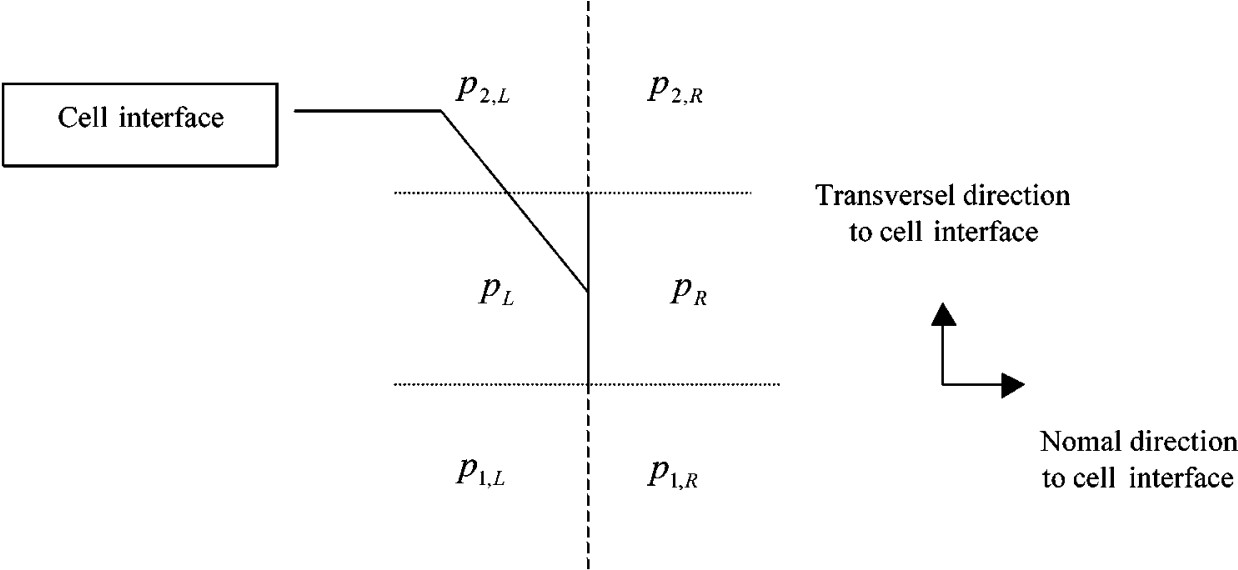
\includegraphics[width=0.75\linewidth]{HW4/ausmpw+.jpg}
    \caption{AUSMPW+ Stencil}
\end{figure}
The Mach number and pressure splitting functions used in the above equations are simplified to the following:
\begin{equation}
    M^\pm =
    \begin{cases}
        \pm\dfrac{1}{4}(M\pm1)^2,& |M| \leq 1\\
        \dfrac{1}{2}(M\pm|M|),& |M|>1
    \end{cases}
\end{equation}
\begin{equation}
    P^\pm|_\alpha =
    \begin{cases}
        \dfrac{1}{4}(M\pm1)^2(2\mp M)\pm\alpha M(M^2-1)^2 ,& |M| \leq 1\\
        \dfrac{1}{2}(1\pm sign(M)) ,& |M| > 1
    \end{cases}
\end{equation}
With the speed of sound calculation done using the following:
\begin{equation}
    \begin{split}
        \dfrac{1}{2}(U_L+U_R) > 0: c_{\frac{1}{2}} = \dfrac{c_s^2}{max(|U_L|,c_s)} \\
        \dfrac{1}{2}(U_L+U_R) < 0: c_{\frac{1}{2}} = \dfrac{c_s^2}{max(|U_R|,c_s)} \\
    \end{split}
\end{equation}
Using:
\begin{equation}
    c_s = \sqrt{\dfrac{2(\gamma-1)}{(\gamma+1)H_{normal}}}
\end{equation}
\begin{equation}
    H_{normal} = 0.5(H_{total,L}-0.5\cdot V_L^2+H_{total,R}-0.5\cdot V_R^2)
\end{equation}
\subsection{AUSM$^+$-up [\texttt{ausm+up}]}
Similar to the previous method, the \textit{AUSM$^+$up} method employs an \textit{advection upstream splitting method} at its core, modifying it to achieve better robustness for low Mach numbers aiming to maintain the convergence rate and accuracy while doing so. (\cite{ausm+up}) In the article, this task is completed by employing an asymptotic analysis under the limit of M$\rightarrow{}$0. This method can be explained as follows: \\
First, define,
\begin{equation}
    M_{L/R}=\dfrac{u_{L/R}}{a_{1/2}}
\end{equation}
With $a_{1/2}$ being defined using the following set of equations:
\begin{equation}
    a_{1/2} = min(\hat{a}_L,\hat{a}_R)
\end{equation}
\begin{equation}
    \begin{split}
        \hat{a}_L&=a^{*2}/max(a^*, u_L) \\
        \hat{a}_R&=a^{*2}/max(a^*, -u_R)
    \end{split}
\end{equation}
\begin{equation}
    a^{*2}=\dfrac{2(\gamma-1)}{\gamma+1}H_t
\end{equation}
Then the split Mach numbers with $\beta=\dfrac{1}{8}$:
\begin{equation}
    \begin{split}
        \mathscr{M}^\pm_{(1)}(M) &= \dfrac{1}{2}(M\pm|M|) \\
        \mathscr{M}^\pm_{(2)}(M) &= \pm\dfrac{1}{4}(M\pm1)^2 \\
        \mathscr{M}^\pm_{(4)}(M) &=
        \begin{cases}
            \mathscr{M}^\pm_{(1)}(M), & |M|\geq1 \\
            \mathscr{M}^\pm_{(2)}(M)(1\mp16\beta\mathscr{M}^\mp_{(2)}(M), & \text{otherwise}
        \end{cases}
    \end{split}
\end{equation}
The split pressure numbers can be defined using the split Mach numbers as the following with $\alpha=\dfrac{3}{16}$:
\begin{equation}
    \mathscr{P}^\pm_{(5)}(M)=
    \begin{cases}
        \dfrac{1}{M}\mathscr{M}^\pm_{(1)}(M), & |M| \geq 1\\
        \mathscr{M}^\pm_{(2)}(M)[(\pm2-M)\mp16\alpha M \mathscr{M}^\mp_{(2)}(M)], & \text{otherwise}
    \end{cases}
\end{equation}
Furthermore, the following are defined:
\begin{equation}
    \bar M^2 = \dfrac{(u_L^2+u_R^2)}{2a^2_{1/2}}
\end{equation}
\begin{equation}
    M_o^2 = min(1, max(\bar M^2, M_\infty^2))
\end{equation}
\begin{equation}
    f_a(M_o) = M_o(2-M_o)
\end{equation}
With $K_p = 0.25$ (which is set as 1 in the \mefvm code) and $\sigma=1$ the following equation yields the interface Mach number with $\rho_{1/2}=0.5(\rho_L+\rho_R)$:
\begin{equation}
    M_{1/2}=\mathscr{M}^+_{(4)}(M_L)+\mathscr{M}^-_{(4)}(M_R)-\dfrac{K_p}{f_a}max(1-\sigma \bar M^2,0)\dfrac{p_R-p_L}{\rho_{1/2}a^2_{1/2}}
\end{equation}
To define the pressure fluxes with $K_u=0.75$ (which set as 1 in the \mefvm code):
\begin{equation}
    \dot m_{1/2}=a_{1/2}M_{1/2}
    \begin{cases}
        \rho_L ,& M_{1/2}>0\\
        \rho_R ,& \text{otherwise}
    \end{cases}
\end{equation}
\begin{equation}
    p_{1/2}=\mathscr{P}^+_{(5)}(M_L)p_L + \mathscr{P}^-_{(5)}(M_R)p_R - K_u\mathscr{P}^+_{(5)}\mathscr{P}^-_{(5)}(\rho_L+\rho_R)(f_aa_{1/2})(u_R-u_L)
\end{equation}
Lastly,
\begin{equation}
    \textbf{f}_{1/2}=\dot m_{1/2}
    \begin{cases}
        \vec{\psi}_L, & \dot m_{1/2}>0\\
        \vec{\psi}_L, & otherwise
    \end{cases}
    + \textbf{p}_{1/2}
\end{equation}
Which mimics the flux function:
\begin{equation}
    \textbf{F}=\textbf{F}^{(c)}+\textbf{P}=\textbf{f}_{1/2}
\end{equation}
\subsection{HLLEM [\texttt{hllem}]} \label{hllem}
The \textit{Harten-Lax-van Leer-Einfeldt} (HLLE) is a positively conservative scheme. The \verb|HLLEM| scheme utilizes a modified Riemann solver. (\cite{hllem}) \\\par
Essentially the \textit{modified HLLE} scheme (\verb|HLLEM|) according to the source is as follows (\cite{hllem}):
\begin{equation}
    \mathbf{\omega}_{HLLEM}(x'/t; i+1/2) = 
    \begin{cases}
        \textbf{v}_i,& x' < b_{i+1/2}^lt \\
        \begin{split}
        \textbf{v}_{i+1/2}+(x-\bar u_{i+1/2}t)(\hat\delta^2_{i+1/2}\hat\alpha^2_{i+1/2}\mathbf{\hat R}^2_{i+1/2}\\+\hat\delta^3_{i+1/2}\hat\alpha^3_{i+1/2}\mathbf{\hat R}^3_{i+1/2})
        \end{split}
        ,& b^l_{i+1/2}<x<b^r_{i+1/2}\\
        \textbf{v}_{i+1/2},& b^r_{1+1/2}<x'
    \end{cases}
\end{equation} \par
\label{avgs}Where $\mathbf{\hat R}^2_{1+1/2}$ and $\mathbf{\hat R}^3_{1+1/2}$ are the 2nd and 3rd eigenvectors of the Jacobian matrix $d\textbf{f}(\mathbf{\hat w_{1+1/2}})=A(\mathbf{\hat w_{1+1/2}})$. Where the required values for $\hat\alpha^2_{i+1/2}$, $\hat\alpha^3_{i+1/2}$ and $\bar u_{i+1/2}$ is found using:
\begin{equation}
    \textbf{v}_{i+1}-\textbf{v}_i=\sum^4_{l=1}\hat\alpha^l_{i+1/2}\mathbf{\hat R}^l_{1+1/2}
\end{equation}
\begin{equation}
    \bar u_{i+1/2}=\dfrac{b^r_{i+1/2}+b^l_{i+1/2}}{2}
\end{equation}
The average state explained \hyperref[avgs]{\textit{here}}, $\mathbf{\hat w_{i+1/2}} = (\hat\rho,\hat u, \hat v, \hat c)^T$ is chosen as:
\begin{equation}
    \hat\rho_{i+1/2}=\sqrt{\rho_i\rho_{i+1/2}}
\end{equation}
\begin{equation}
    \hat u_{i+1/2}=\dfrac{\sqrt{\rho_i}u_i+\sqrt{\rho_{i+1}}u_{i+1}}{\sqrt{\rho_i}+\sqrt{\rho_{i+1}}}
\end{equation}
\begin{equation}
    \hat v_{i+1/2}=\dfrac{\sqrt{\rho_i}v_i+\sqrt{\rho_{i+1}}v_{i+1}}{\sqrt{\rho_i}+\sqrt{\rho_{i+1}}}
\end{equation}
\begin{equation}
    \hat H_{i+1/2}=\dfrac{\sqrt{\rho_i}H_i+\sqrt{\rho_{i+1}}H_{i+1}}{\sqrt{\rho_i}+\sqrt{\rho_{i+1}}}
\end{equation}
\begin{equation}
    \hat c^2_{i+1/2}=(\gamma-1)\left[ H_{i+1/2}-\dfrac{1}{2}(u_{i+1/2}^2+v_{i+1/2}^2)\right]
\end{equation}
The modified version defines the $\delta^2_{i+1/2}$ and $\delta^3_{i+1/2}$ as the following in order to take out excess dissipation (\cite{hllem}):
\begin{equation}
    \delta^2_{i+1/2}=\delta^3_{i+1/2}=\dfrac{\hat c_{i+1/2}}{\hat c_{i+1/2}+|\bar u_{i+1/2}|}
\end{equation}
With $b^l_{i+1/2}$ and $b^r_{i+1/2}$ being defined as the largest and the smallest eigenvalues of the Roe-average matrix. (\cite{hllem}) The HLLEM scheme is written as:
\begin{equation}
    \textbf{f}_{i+1/2}=\dfrac{1}{2}\left[\textbf{f}(\textbf{v}_i)+\textbf{f}(\textbf{v}_{i+1})-\sum^4_{R=1}Q_{i+1/2}^R\alpha_{i+1/2}^RR_{i+1/2}^R\right]
\end{equation}
\begin{equation}
    Q^1_{i+1/2} = \dfrac{b^+_{i+1/2}+b^-_{i+1/2}}{b^+_{i+1/2}-b^-_{i+1/2}}\alpha^1_{i+1/2}-2\dfrac{b^+_{i+1/2}b^-_{i+1/2}}{b^+_{i+1/2}-b^-_{i+1/2}}
\end{equation}
\begin{equation}
    Q^2_{i+1/2}=\dfrac{b^+_{i+1/2}+b^-_{i+1/2}}{b^+_{i+1/2}-b^-_{i+1/2}}\alpha^2_{i+1/2}-2(1-\delta^2_{i+1/2})\dfrac{b^+_{i+1/2}b^-_{i+1/2}}{b^+_{i+1/2}-b^-_{i+1/2}}
\end{equation}
\begin{equation}
    Q^3_{i+1/2}=\dfrac{b^+_{i+1/2}+b^-_{i+1/2}}{b^+_{i+1/2}-b^-_{i+1/2}}\alpha^3_{i+1/2}-2(1-\delta^3_{i+1/2})\dfrac{b^+_{i+1/2}b^-_{i+1/2}}{b^+_{i+1/2}-b^-_{i+1/2}}
\end{equation}
\begin{equation}
    Q^4_{i+1/2} = \dfrac{b^+_{i+1/2}+b^-_{i+1/2}}{b^+_{i+1/2}-b^-_{i+1/2}}\alpha^4_{i+1/2}-2\dfrac{b^+_{i+1/2}b^-_{i+1/2}}{b^+_{i+1/2}-b^-_{i+1/2}}
\end{equation}\par
\mefvm implements this method a bit differently than explained here similar to the \hyperref[roe]{\textit{Roe method}}. It was quite hard to understand this implementation due to a lack of background knowledge and inconsistent notation schemes across different articles. 
\subsection{Rusanov [\texttt{rusanov}]}
Nostalgia from homework 3 (\cite{hw3}), Rusanov uses "through" calculation schemes in Eulerian coordinates aiming to reduce the tangential discontinuities for 2-dimensional problems. (\cite{rusanov})\par
First Rusanov starts by defining the following:
\begin{equation}
    \dfrac{\partial f}{\partial t}+\dfrac{\partial F^x}{\partial x}+\dfrac{\partial F^y}{\partial y}+ \Psi = 0
\end{equation}
Where:
\begin{equation}
    f=\begin{Bmatrix}
        \rho\\r\\s\\e
    \end{Bmatrix},\:
    F^x=\begin{Bmatrix}
        r\\p+ru\\rv\\(e+p)u
    \end{Bmatrix},\:
    F^y=\begin{Bmatrix}
        s\\su\\p+sv\\(e+p)v
    \end{Bmatrix},\:
    \Psi=\dfrac{\nu v}{y}\begin{Bmatrix}
        \rho\\r\\s\\e+p
    \end{Bmatrix}
\end{equation}
With $\nu = 0$ for plane flow, $\nu = 1$ if there is axial symmetry. Furthermore:
\begin{equation}
    r = \rho u,\: s= \rho v,\: e=\dfrac{\rho(u^2+v^2)}{2}+\dfrac{p}{k-1}
\end{equation}
Rusanov then defines:
\begin{equation}
    \phi = \begin{Bmatrix}
        u\\v\\p\\\rho
    \end{Bmatrix},\: w=\sqrt{u^2+v^2},\: c=\sqrt{\dfrac{kp}{\rho}}
\end{equation}
With simple trigonometric expression for boundary interfaces. Rusanov then moves on to define the difference with $\Delta x = h_1$, $\Delta y=h_2$, and $\Delta t=r$. Furthermore, the value of any quantity, a, at a point with coordinates ($mh_1$, $lh_2$, $nr$) is denoted as $a_{m,l}^n$
\begin{equation}
    h = \sqrt{h_1^2+h_2^2},\: x_i = \dfrac{\tau}{h_i},\: x=\sqrt{x_1^2+x_2^2}
\end{equation}
Then Rusanov defines the following:
\begin{equation}
\begin{split}    
    \Phi^x_{m+1/2,l}=\alpha^n_{m+1/2,l}(f_{m+1,1}-f_{m,l})^n,&\:\alpha^n_{m+1/2,l}=\dfrac{1}{2}(\alpha_{m+1,l}+\alpha_{m,l})^n \\
    \Phi^y_{m,l+1/2}=\beta^n_{m,l+1/2}(f_{m+1,1}-f_{m,l})^n,&\:\beta^n_{m,l+1/2}=\dfrac{1}{2}(\beta_{m,l+1}+\beta_{m,l})^n \\
    \alpha^n_{m,l}=\omega x(w+c)^n_{m,l}sin^2X,&\:\beta^n_{m,l}=\omega x(w+c)^n_{m,l}cos^2X
\end{split}
\end{equation}
There are several stability conditions Rusanov states but suggests to use $\alpha^n_{m,l}=\beta^n_{m,l}=\dfrac{1}{2}$. After some further reductions, the numerical flux becomes (\cite{rusanov}):
\begin{equation}
    f^{n+1}_{m,0}=f^n_{m,0}-\tau\hat\Psi^n_{m,0}-\dfrac{x_1}{2}(F^x_{m+1,0}-F^x_{m-1,0})-x_2F^{yn}_{m,1}+\dfrac{1}{2}(\Phi^x_{m+1/2,0}-\Phi^x_{m-1/2,0}+2\Phi^y_{m,1/2})
\end{equation}\par
\mefvm utilizes a more concise code similar to the code written in Homework 3 (\cite{hw3}). \\\par
A table is shared below which compares all the advantages and disadvantages of the methods.
\begin{table}[h]
    \renewcommand\baselinestretch{1.1}\selectfont
    \centering
    \mbox{}\clap{
    \begin{tblr}
        []{
        rowsep =1mm,
        colspec = {Q[c,m, 5cm]Q[c,m,5cm]Q[c,m,5cm]},
        vlines, hlines,
        row{1} = {gray9}
        }
        Method name & Advantages & Disadvantages\\
        {Roe [roe]} & {Accurate modeling of shocks and contact discontinuities. Suitable for high-speed flows and shock structures.} & {Instability in low-speed regimes. Risk of producing non-physical solutions.}\\
        
        RoeM [roem] & {Stability in low-speed problems. More accurate results in low-speed regions (e.g., post-shock areas).} & {May not provide as sharp solutions as classic Roe in high-speed regimes.}\\
        
        Rotated-RoeM [rotated-roem]& {Accurate resolution of oblique shocks and complex flow structures. Ideal for oblique flows in scramjet inlets.} & {Higher computational cost compared to Roe and RoeM.}\\
        
        AUSMPW+ [ausmpw+]& {High resolution in shock and separation regions. High accuracy in aero-dynamic analyses.} & {High computational cost.}\\
        
        $\text{AUSM}^+\text{-up}$ [ausm+up]& {Stable solutions at low Mach numbers. Accurate modeling of shock waves and separations.} & {Potential loss of accuracy in high-speed flows compared to other methods.}\\   
        
        HLLEM [hllem]& {Stable resolution of shocks and contact discontinuities. Provides more stability.} & {Diffusive tendency leading to loss of resolution.}\\ 
        
        Rusanov [rusanov]& {Simple and fast method.} & {Low accuracy in shocks and contact discontinuities.}\\ 
    
    \end{tblr}
    }
    \caption{Comparison of Numerical Flux Functions}
    \label{ap2}
\end{table}
\newpage
Though not explained in detail in the previous section, a table was created comparing the different time discretization schemes:
\begin{table}[H]
    \renewcommand\baselinestretch{1.1}\selectfont
    \centering
    \mbox{}\clap{
    \begin{tblr}
        []{
        rowsep =1mm,
        colspec = {Q[c,m, 6.5cm]Q[c,m,6.5cm]},
        vlines, hlines,
        row{1} = {gray9}
        }
        LU-SGS & TVD-RK3 \\
        Efficient for steady-state solutions in both subsonic and supersonic flows. & Suitable for transient solutions in both subsonic and supersonic flows. \\
        Requires fewer iterations for steady-state convergence, making it ideal for subsonic and steady supersonic flows. & Provides high-order accuracy, especially useful for resolving transient phenomena in both regimes. \\
        Handles stiff nonlinearity effectively, making it robust for supersonic shock interactions. & Excels in resolving sharp gradients and discontinuities, such as shocks in supersonic flows. \\ 
        Computational cost is higher due to matrix operations but fewer time steps are required. & Computational cost per step is lower but requires more time steps due to stability constraints, especially in subsonic flows. \\
        Well-suited for steady subsonic flows and steady supersonic shock-dominated problems. & Performs better for time-dependent subsonic and supersonic flows, such as unsteady shock oscillations. \\
        Memory requirements are relatively low due to its iterative nature. & Higher memory requirements because of intermediate stages in each time step. \\
        Less flexible for complex boundary conditions in subsonic flows. & More flexible for implementing complex boundary conditions, especially in subsonic regimes.
    
    \end{tblr}
    }
    \caption{Comparison of LU-SGS and TVD-RK3 Methods for Subsonic and Supersonic Flow Solutions (\cite{lu}, \cite{tvd})}
    \label{ap2}
\end{table}
\newpage
\section{Explanation of the Benchmark Problems}

\subsection{Forward Facing Slope}
In the figures and table below, the domain and boundary conditions to be used for forward-facing benchmark are shown. This benchmark includes a right-moving Mach 3 fluid entering a wind tunnel, which reduces its height due to a step opposing the direction of the fluid. \par
In this benchmark problem, before starting the meshing process, it is known that there will be a shock around the 3rd wall. Therefore, applying a finer mesh to the area around the 3rd wall is of great importance for the accuracy of the solution. 
\begin{figure}[H]
    \centering
    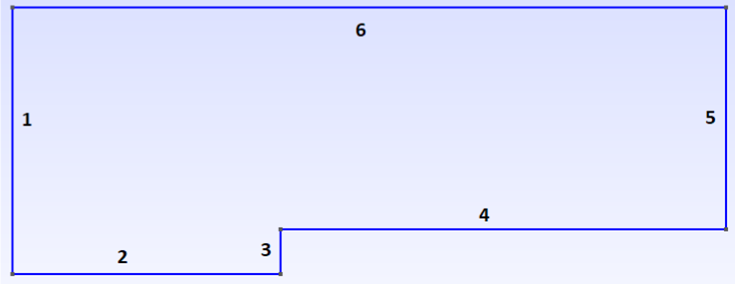
\includegraphics[width=1\linewidth]{HW4/Forward facing step Benchmark Domain (M=3).png}
    \caption{Forward facing step Benchmark Domain (M=3)}
\end{figure}

\begin{table}[H]
    \renewcommand\baselinestretch{1.1}\selectfont
    \centering
    \mbox{}\clap{
    \begin{tblr}
        []{
        rowsep =1mm,
        colspec = {Q[c,m, 3cm]Q[c,m,5cm]},
        vlines, hlines,
        row{1} = {gray9}
        }
        Face Number & Boundary Condition\\
        1 & Supersonic\\
        2 & Slip Wall\\
        3 & Slip Wall\\
        4 & Slip Wall\\
        5 & Subsonic Pressure Outflow\\
        6 & Slip Wall\\
    \end{tblr}
    }
    \caption{Boundary Conditions}
\end{table}

The meshes produced for the Forward Facing Step benchmark are in the figures below.

\begin{figure}[H]
    \centering
    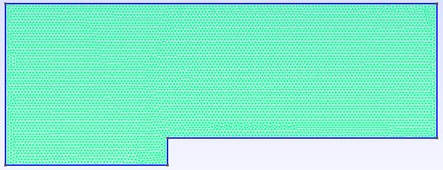
\includegraphics[width=1\linewidth]{HW4/Forward facing step triangular.png}
    \caption{Forward facing step triangular}
\end{figure}
\begin{figure}[H]
    \centering
    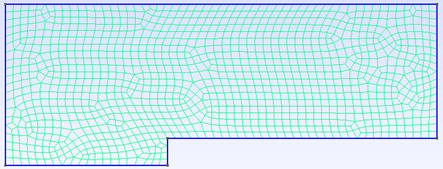
\includegraphics[width=1\linewidth]{HW4/Forward facing step quadrilateral.png}
    \caption{Forward facing step quadrilateral}
\end{figure}
\begin{figure}[H]
    \centering
    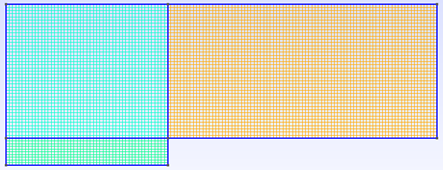
\includegraphics[width=1\linewidth]{HW4/Forward facing step structural.png}
    \caption{Forward facing step structural}
\end{figure}

\begin{table}[H]
    \renewcommand\baselinestretch{1.1}\selectfont
    \centering
    \mbox{}\clap{
    \begin{tblr}
        []{
        rowsep =1mm,
        colspec = {Q[c,m, 4cm]Q[c,m,4cm]Q[c,m,4cm]},
        vlines, hlines,
        row{1} = {gray9}
        }
        Mesh name &  Node Amount & Element Amount\\
        Forward facing step triangular & 7268  & 14540\\
        Forward facing step quadrilateral & 1249 & 1329\\
        Forward facing step structural & 6315 & 6600 \\
    \end{tblr}
    }
    \caption{ Mesh Properties of Forward-facing step benchmark}
\end{table}
As can be seen from the table above, although the node numbers are very close to each other for “Forward facing step triangular” and “Forward facing step structural” there are almost twice as many elements in "Forward facing step triangular".  Furthermore, there are much fewer nodes and elements in the quadrilateral mesh than in the other two meshes. Therefore, it is expected that the analyses performed using "Forward facing step triangular" will be relatively more successful and accurate.\\\par

In the supersonic forward-facing step benchmark, flux functions must handle strong shocks, expansion waves, and complex flow features like shock-shock and shock-boundary layer interactions. $\text{AUSM}^+\text{-up}$ and AUSMPW+ are expected to yield the most accurate results due to their robust shock-capturing capability, low dissipation, and ability to resolve sharp flow features. Rotated-RoeM and RoeM also perform well, providing good resolution of oblique shocks and minimizing numerical artifacts in regions with strong gradients. The Roe solver is effective but may require entropy fixes to handle instabilities near shock interactions. HLLM offers robustness and stability but introduces excessive diffusion, which reduces the resolution of key flow structures. Rusanov is the least suitable, as its high dissipation smears shocks and fails to resolve intricate features accurately in such a challenging supersonic flow scenario.


\subsection{Flow Over a Circular Bump}
In the figures and table below, the domain and boundary conditions to be used for the flow over a circular bump benchmark are shown. This benchmark problem examines transonic and supersonic flows over a bump within a channel geometry. For the transonic case, the circular bump on the lower wall has a thickness equal to 10\% of its length, whereas, for the supersonic case, the arc-shaped bump’s thickness is reduced to 4\% of its length. \par
In this benchmark problem, before starting the meshing process, it is known that there will most likely be a shock on the circular bump in the supersonic case. Therefore, applying a finer mesh to the area above the circular bump is of great importance for the accuracy of the solution.\\

\begin{figure}[H]
    \centering
    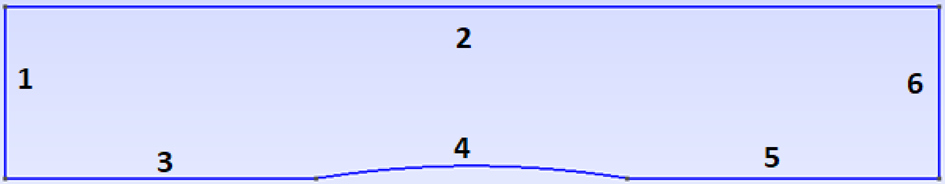
\includegraphics[width=1\linewidth]{HW4/Supersonic Flow over a Circular Bump Domain M_1=1.4.png}
    \caption{Supersonic Flow over a Circular Bump Domain $M_1$=1.4}
\end{figure}

\begin{figure}[H]
    \centering
    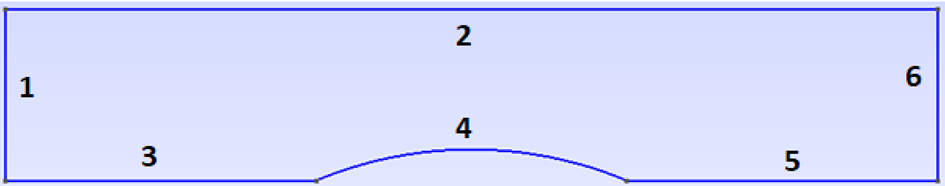
\includegraphics[width=1\linewidth]{HW4/Transonic Flow over a Circular Bump Domain M_1=0.675.png}
    \caption{Transonic Flow over a Circular Bump Domain $M_1$=0.675}
\end{figure}

\begin{table}[H]
    \renewcommand\baselinestretch{1.1}\selectfont
    \centering
    \mbox{}\clap{
    \begin{tblr}
        []{
        rowsep =1mm,
        colspec = {Q[c,m, 3cm]Q[c,m,5cm]},
        vlines, hlines,
        row{1} = {gray9}
        }
        Face Number & Boundary Condition\\
        1 & Supersonic/Transonic Inlet\\
        2 & Slip Wall\\
        3 & Slip Wall\\
        4 & Slip Wall\\
        5 & Slip Wall\\
        6 & Subsonic Pressure Outflow\\
    \end{tblr}
    }
    \caption{Boundary Conditions}
\end{table}
The meshes produced for the supersonic case are shown in the figures below.

\begin{figure}[H]
    \centering
    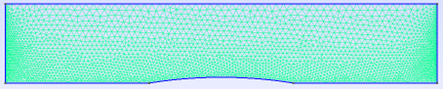
\includegraphics[width=1\linewidth]{HW4/Supersonic flow over a circular bump mesh 1.png}
    \caption{Supersonic flow over a circular bump mesh 1}
\end{figure}


\begin{figure}[H]
    \centering
    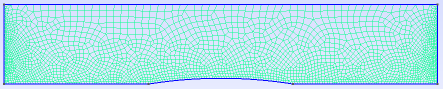
\includegraphics[width=1\linewidth]{HW4/Supersonic flow over a circular bump mesh 2.png}
    \caption{Supersonic flow over a circular bump mesh 2}
\end{figure}

As can be seen in the figures above, the circular bump is more finely meshed than the rest of the domain in both meshes. The purpose of choosing these two mesh types in this benchmark test is to determine the effect of triangular and quadrilateral mesh geometries on the obtained residual values.

\begin{table}[H]
    \renewcommand\baselinestretch{1.1}\selectfont
    \centering
    \mbox{}\clap{
    \begin{tblr}
        []{
        rowsep =1mm,
        colspec = {Q[c,m, 4cm]Q[c,m,4cm]Q[c,m,4cm]},
        vlines, hlines,
        row{1} = {gray9}
        }
        Mesh name &  Node Amount & Element Amount\\
        Supersonic flow over a circular bump mesh 1 & 3167 & 6337\\
        Supersonic flow over a circular bump mesh 2 & 3090  & 3274 \\
    \end{tblr}
    }
    \caption{Mesh Properties of Transonic Flow Over a Circular Bump Benchmark}
\end{table}

As can be seen from the table above, although the node numbers are very close to each other, there are almost twice as many elements in "Transonic flow over a circular bump mesh 1". Therefore, it is expected that the analyses made using "Transonic flow over a circular bump mesh 1" will be relatively more successful and accurate.\\\par
In the transonic flow over a circular bump benchmark, the performance of flux functions is determined by their ability to handle mixed subsonic and supersonic regions, including shock-boundary layer interactions. $\text{AUSM}^+\text{-up}$ and AUSMPW+ are expected to perform best, offering an accurate resolution of shocks and smooth transitions between flow regimes. RoeM and Rotated-RoeM are also strong contenders, effectively capturing shocks and mitigating instabilities near sonic points. The Roe solver provides reasonable results but may require entropy fixes to avoid nonphysical solutions in sonic regions. HLLM delivers robust but slightly diffusive solutions, resulting in less precise shock resolution. Rusanov performs poorly due to its high dissipation, which smears shocks and smooths critical flow features, making it unsuitable for high-resolution transonic benchmarks.\\\par

The meshes produced for the transonic case are shown in the figures below.

\begin{figure}[H]
    \centering
    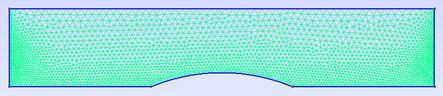
\includegraphics[width=1\linewidth]{HW4/Transonic flow over a circular bump mesh 1.png}
    \caption{Transonic Flow Over a Circular Bump Mesh 1}
\end{figure}
\begin{figure}[H]
    \centering
    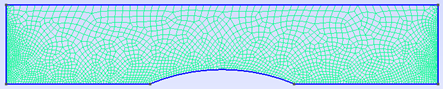
\includegraphics[width=1\linewidth]{HW4/Transonic flow over a circular bump mesh 2.png}
    \caption{Transonic Flow Over a Circular Bump Mesh 2}
\end{figure}

As can be seen in the figures above, the circular bump is more finely meshed than the rest of the domain in both meshes. The purpose of choosing these two mesh types in this benchmark test is to determine the effect of triangular and quadrilateral mesh geometries on the obtained residual values.

\begin{table}[H]
    \renewcommand\baselinestretch{1.1}\selectfont
    \centering
    \mbox{}\clap{
    \begin{tblr}
        []{
        rowsep =1mm,
        colspec = {Q[c,m, 4cm]Q[c,m,4cm]Q[c,m,4cm]},
        vlines, hlines,
        row{1} = {gray9}
        }
        Mesh name &  Node Amount & Element Amount\\
        Transonic flow over a circular bump mesh 1 & 3173 & 6349\\
        Transonic flow over a circular bump mesh 2 & 3102  & 3286 \\
    \end{tblr}
    }
    \caption{Mesh Properties of Transonic Flow Over a Circular Bump Benchmark}
\end{table}

As can be seen from the table above, although the node numbers are very close to each other, there are almost twice as many elements in "Transonic flow over a circular bump mesh 1". Therefore, it is expected that the analyses made using "Transonic flow over a circular bump mesh 1" will be relatively more successful and accurate.\\\par
In the transonic flow over a circular bump benchmark, the performance of flux functions is determined by their ability to handle mixed subsonic and supersonic regions, including shock-boundary layer interactions. $\text{AUSM}^+\text{-up}$ and AUSMPW+ are expected to perform best, offering an accurate resolution of shocks and smooth transitions between flow regimes. RoeM and Rotated-RoeM are also strong contenders, effectively capturing shocks and mitigating instabilities near sonic points. The Roe solver provides reasonable results but may require entropy fixes to avoid nonphysical solutions in sonic regions. HLLM delivers robust but slightly diffusive solutions, resulting in less precise shock resolution. Rusanov performs poorly due to its high dissipation, which smears shocks and smooths critical flow features, making it unsuitable for high-resolution transonic benchmarks.


\subsection{Scramjet Inlet Flow Model with Different Boundary Conditions}
The geometry, domain, and boundary conditions for the scramjet inlet flow model benchmark are given in the figure below. In this benchmark, a flow flowing at Mach 3 is simulated encountering an obstacle while passing through a converging channel.

\begin{figure}[H]
    \centering
    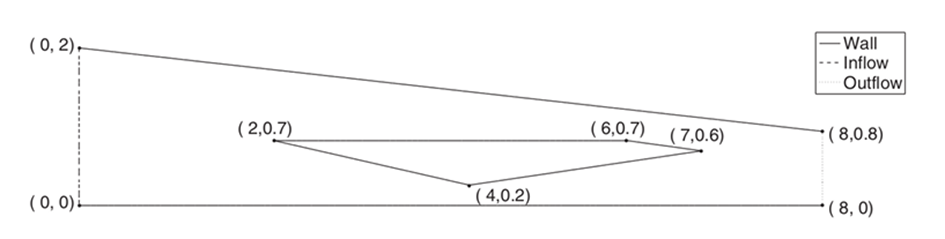
\includegraphics[width=1\linewidth]{HW4/scramjet inlet .png}
    \caption{Sketch of the domain and the boundary conditions used in scramjet inlet model case}
\end{figure}

Before starting the mesh creation process, it is necessary to note that in a supersonic flow, any obstacle is very likely to create shock in the region where the obstacle is located. Therefore, a finer mesh should be created in order to get better results in the areas expected to be shocked. The meshes applied in this regard are shown in the figures below. 

\begin{figure}[H]
    \centering
    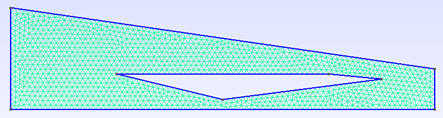
\includegraphics[width=1\linewidth]{HW4/Scramjet inlet flow model mesh 1.png}
    \caption{Scramjet inlet flow model mesh 1}
\end{figure}

\begin{figure}[H]
    \centering
    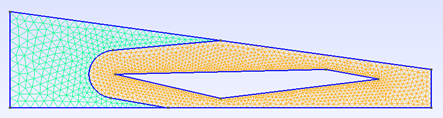
\includegraphics[width=1\linewidth]{HW4/Scramjet inlet flow model mesh 2.png}
    \caption{Scramjet inlet flow model mesh 2}
\end{figure}

In both Figure 2 and Figure 3, the boundary conditions are assigned as shown in Figure 1, and the geometric dimensions are exactly the same. In the mesh shown in Figure 2, the entire domain is meshed with triangular mesh elements, with a finer mesh applied only to areas very close to the obstacle. The other mesh in Figure 3 is again composed entirely of triangular meshes, but a finer mesh is applied to include the entire surrounding of the obstacle.

\begin{table}[H]
    \renewcommand\baselinestretch{1.1}\selectfont
    \centering
    \mbox{}\clap{
    \begin{tblr}
        []{
        rowsep =1mm,
        colspec = {Q[c,m, 4cm]Q[c,m,4cm]Q[c,m,4cm]},
        vlines, hlines,
        row{1} = {gray9}
        }
        Mesh name &  Node Amount & Element Amount\\
        Scramjet inlet flow model mesh 1 & 1341 & 2690\\
        Scramjet inlet flow model mesh 2 & 1789 & 3638\\
    \end{tblr}
    }
    \caption{Mesh Properties of Scramjet inlet flow model benchmark}
\end{table}

Considering the discarded meshes and the nature of the problem, the residual values obtained in "Scramjet inlet flow model mesh 2" are generally expected to be lower than the residual values obtained in "Scramjet inlet flow model mesh 1". The main reason for this is that while only the sharp changes caused by shock in the regions very close to the obstacle can be detected in "Scramjet inlet flow model mesh 1", on the other hand, all sharp changes caused by sock formed around the obstacle can be detected in "Scramjet inlet flow model mesh 2". This allows us to expect the residuals obtained in "Scramjet inlet flow model mesh 2" to be lower.\\\par
In this benchmark problem, all computations are done on the residual of the density, and some of the flux functions mentioned above are expected to yield better results than others. For density residual calculations, $\text{AUSM}^+\text{-up}$ and Rotated-RoeM are expected to yield the best results due to their superior shock resolution, low dissipation, and robustness in handling compressible flows. AUSMPW+ is also a strong choice, particularly in scenarios with complex shock and expansion wave interactions. The standard Roe solver and RoeM perform well but may require adjustments to mitigate instabilities. HLLM and Rusanov, while robust, are less favorable for achieving accurate density residuals in such applications.

\section{Tests and Results}
In this section of the report, relative tests of numerical flux functions and their results will be shared and discussed.\\\par

As an early warning, the initial condition and the outflow pressure are constant among the tested meshes and benchmark problems. The residual $\rho$ for every test case can be found in the tables below.

\begin{table}[H]
    \renewcommand\baselinestretch{1.1}\selectfont
    \centering
    \mbox{}\clap{
    \begin{tblr}
        []{
        rowsep =1mm,
        colspec = {Q[c,m, 2.5cm]Q[c,m,2cm]Q[c,m,2cm]Q[c,m,2cm]Q[c,m,2cm]Q[c,m,2cm]Q[c,m,2cm]},
        vlines, hlines,
        row{1} = {gray9},
        cell{1}{1} = {r=2}{c},
        cell{1}{2,4,6} = {c=2}{c}
        }
        Method Name & Triangular & & Quadrilateral & & Structured & \\
         & lu-sgs & tvd-rk3 & lu-sgs & tvd-rk3 & lu-sgs & tvd-rk3\\
        roe & {0.09712} & {0.07654} & {0.01615} & {0.02866} & {0.10387} & {0.15758}\\
        roem & {0.02318} & {0.02031} & {0.00776} & {0.01219} & {0.07344} & {0.08949}\\
        rotated-roem & {0.00604} & {0.00529} & {0.03302} & {0.01605} & {0.03912} & {0.04148}\\
        ausmpw+ & {0.01251} & {0.01244} & {0.04079} & {0.05024} & {0.08107} & {0.08308}\\
        ausm+up & {0.25721} & {0.38676} & {0.09322} & {0.12029} & {0.06009} & {0.08723}\\
        hllem & {0.05009} & {0.06961} & {0.04653} & {0.03131} & {0.11251} & {0.14553}\\
        rusanov & {0.00350} & {0.00988} & {0.01404} & {0.01206} & {0.02524} & {0.03009}\\
    \end{tblr}
    }
    \caption{Results for Forward Facing Step Triangular \& Quadrilateral \& Structured}
\end{table}

\begin{table}[H]
    \renewcommand\baselinestretch{1.1}\selectfont
    \centering
    \mbox{}\clap{
    \begin{tblr}
        []{
        rowsep =1mm,
        colspec = {Q[c,m, 2.5cm]Q[c,m,2cm]Q[c,m,2cm]Q[c,m,2cm]Q[c,m,2cm]},
        vlines, hlines,
        row{1} = {gray9},
        cell{1}{1} = {r=2}{c},
        cell{1}{2,4} = {c=2}{c}
        }
        Method Name & Mesh 1 & & Mesh 2 & \\
         & lu-sgs & tvd-rk3 & lu-sgs & tvd-rk3\\
        roe & {0.00285} & {0.00375} & {0.03130} & {0.03817}\\
        roem & {0.00279} & {0.00394} & {0.00416} & {0.00652}\\
        rotated-roem & {0.00010} & {0.00010} & {0.00973} & {0.01317}\\
        ausmpw+ & {0.00245} & {0.00284} & {0.01528} & {0.02141}\\
        ausm+up & {0.00303} & {0.00429} & {0.03651} & {0.05332}\\
        hllem & {0.00448} & {0.00465} & {0.02886} & {0.03445}\\
        rusanov & {0.00298} & {0.00635} & {0.00267} & {0.00362}\\
    \end{tblr}
    }
    \caption{Results for Supersonic flow over a circular bump mesh 1 \& 2}
\end{table}

\begin{table}[H]
    \renewcommand\baselinestretch{1.1}\selectfont
    \centering
    \mbox{}\clap{
    \begin{tblr}
        []{
        rowsep =1mm,
        colspec = {Q[c,m, 2.5cm]Q[c,m,2cm]Q[c,m,2cm]Q[c,m,2cm]Q[c,m,2cm]},
        vlines, hlines,
        row{1} = {gray9},
        cell{1}{1} = {r=2}{c},
        cell{1}{2,4} = {c=2}{c}
        }
        Method Name & Mesh 1 & & Mesh 2 & \\
         & lu-sgs & tvd-rk3 & lu-sgs & tvd-rk3\\
        roe & {0.00010} & {0.00010} & {0.01269} & {0.04222}\\
        roem & {0.00087} & {0.00103} & {0.02406} & {0.04275}\\
        rotated-roem & {0.00010} &  {0.00010} & {0.0080} & {0.01440}\\
        ausmpw+ & {0.00516} & {0.00634} & {0.01146} & {0.01206}\\
        ausm+up & {0.00597} & {0.00651} & {0.00931} & {0.02012}\\
        hllem & {0.00010} & {0.00013} & {0.02095} & {0.03391}\\
        rusanov & {0.00042} & {0.00089} & {0.00653} & {0.00674}\\
    \end{tblr}
    }
    \caption{Results for Transonic flow over a circular bump mesh 1 \& 2}
\end{table}

\begin{table}[H]
    \renewcommand\baselinestretch{1.1}\selectfont
    \centering
    \mbox{}\clap{
    \begin{tblr}
        []{
        rowsep =1mm,
        colspec = {Q[c,m, 2.5cm]Q[c,m,2cm]Q[c,m,2cm]Q[c,m,2cm]Q[c,m,2cm]},
        vlines, hlines,
        row{1} = {gray9},
        cell{1}{1} = {r=2}{c},
        cell{1}{2,4} = {c=2}{c}
        }
        Method Name & Mesh 1 & & Mesh 2 & \\
         & lu-sgs & tvd-rk3 & lu-sgs & tvd-rk3\\
        roe & {0.04769} & {0.00375} & {0.04333} & {0.01543}\\
        roem & {0.00051} & {0.00076} & {0.00074} & {0.00505}\\
        rotated-roem & {0.00994} & {0.01041} & {0.00025} & {0.00354}\\
        ausmpw+ & {0.00785} & {0.03689} & {0.00298} & {0.00504}\\
        ausm+up & {0.05614} & {0.07210} & {0.10301} & {0.10275}\\
        hllem & {0.01647} & {0.00877} & {0.00075} & {0.00836}\\
        rusanov & {0.00298} & {0.00635} & {0.00384} & {0.00133}\\
    \end{tblr}
    }
    \caption{Results for Scramjet Inlet Flow Benchmark with Mesh 1 \& 2}
\end{table}


\par
For the sake of simplicity of the commentary, all of the residuals will be plotted. In addition, the table shared below is a coding in which each method is paired with a number starting from one. The following figures are a comparison of all the residuals shared.

\begin{table}[H]
    \renewcommand\baselinestretch{1.1}\selectfont
    \centering
    \mbox{}\clap{
    \begin{tblr}
        []{
        rowsep =1mm,
        colspec = {Q[c,m, 3cm]Q[c,m,2cm]},
        vlines, hlines,
        row{1} = {gray9}
        }
        Corresponding Method & Encryption Number\\
        roe & 1\\
        roem & 2\\
        rotated-roem & 3\\
        ausmpw+ & 4\\
        ausm+up & 5\\
        hllem & 6\\
        rusanov & 7\\
        
    \end{tblr}
    }
    \caption{Mesh Properties of Scramjet inlet flow model benchmark}
\end{table}

\begin{figure}[H]
    \centering
    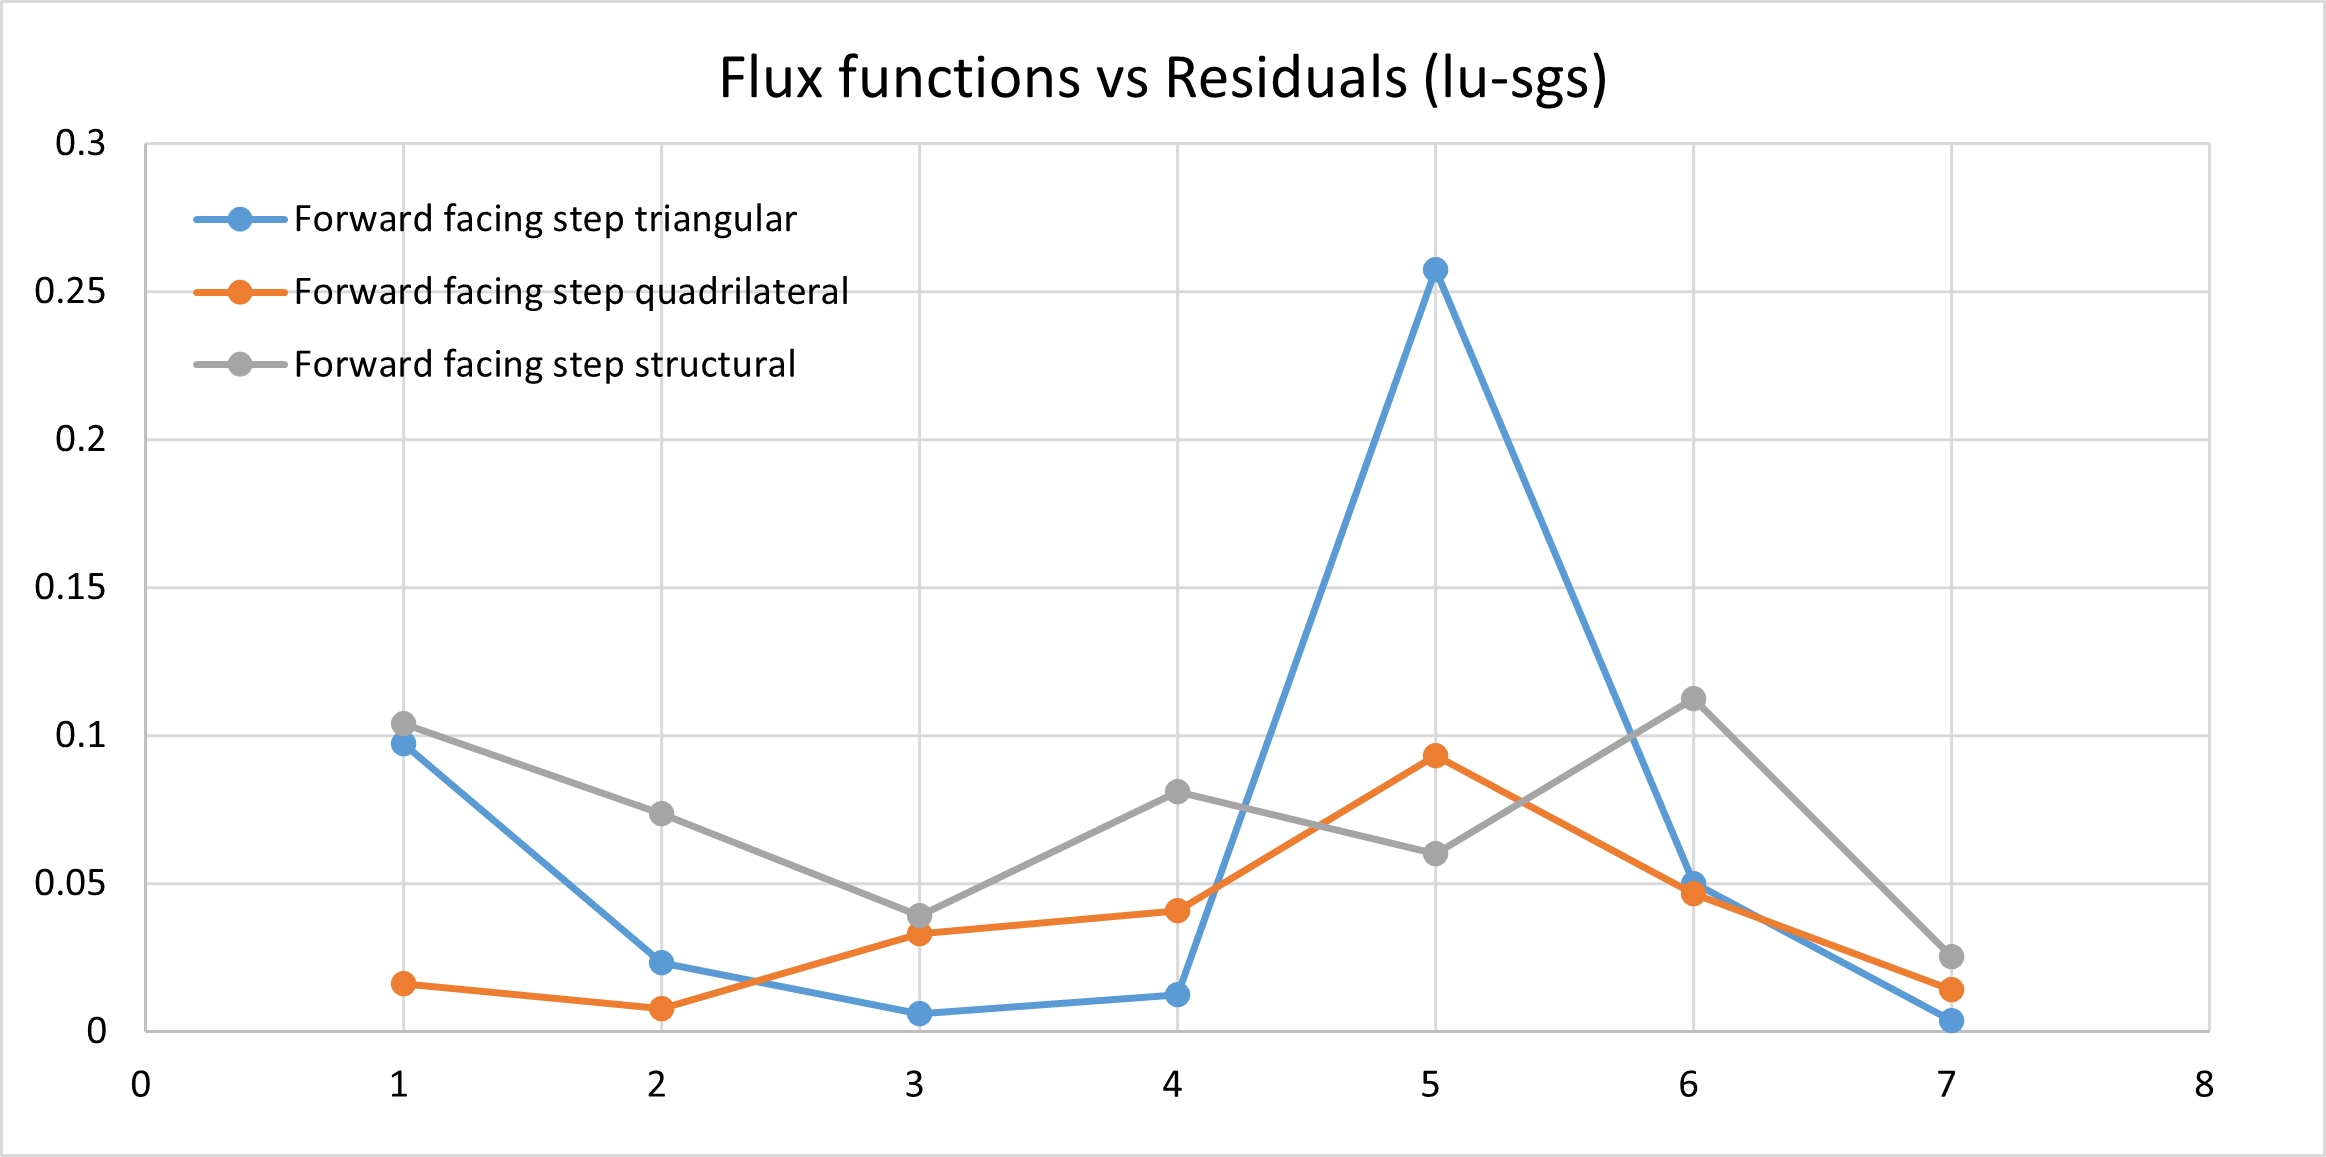
\includegraphics[width=0.75\linewidth]{HW4/lu-sgs Forward Facing.png}
    \caption{Forward Facing Step lu-sgs}
\end{figure}
\begin{figure}[H]
    \centering
    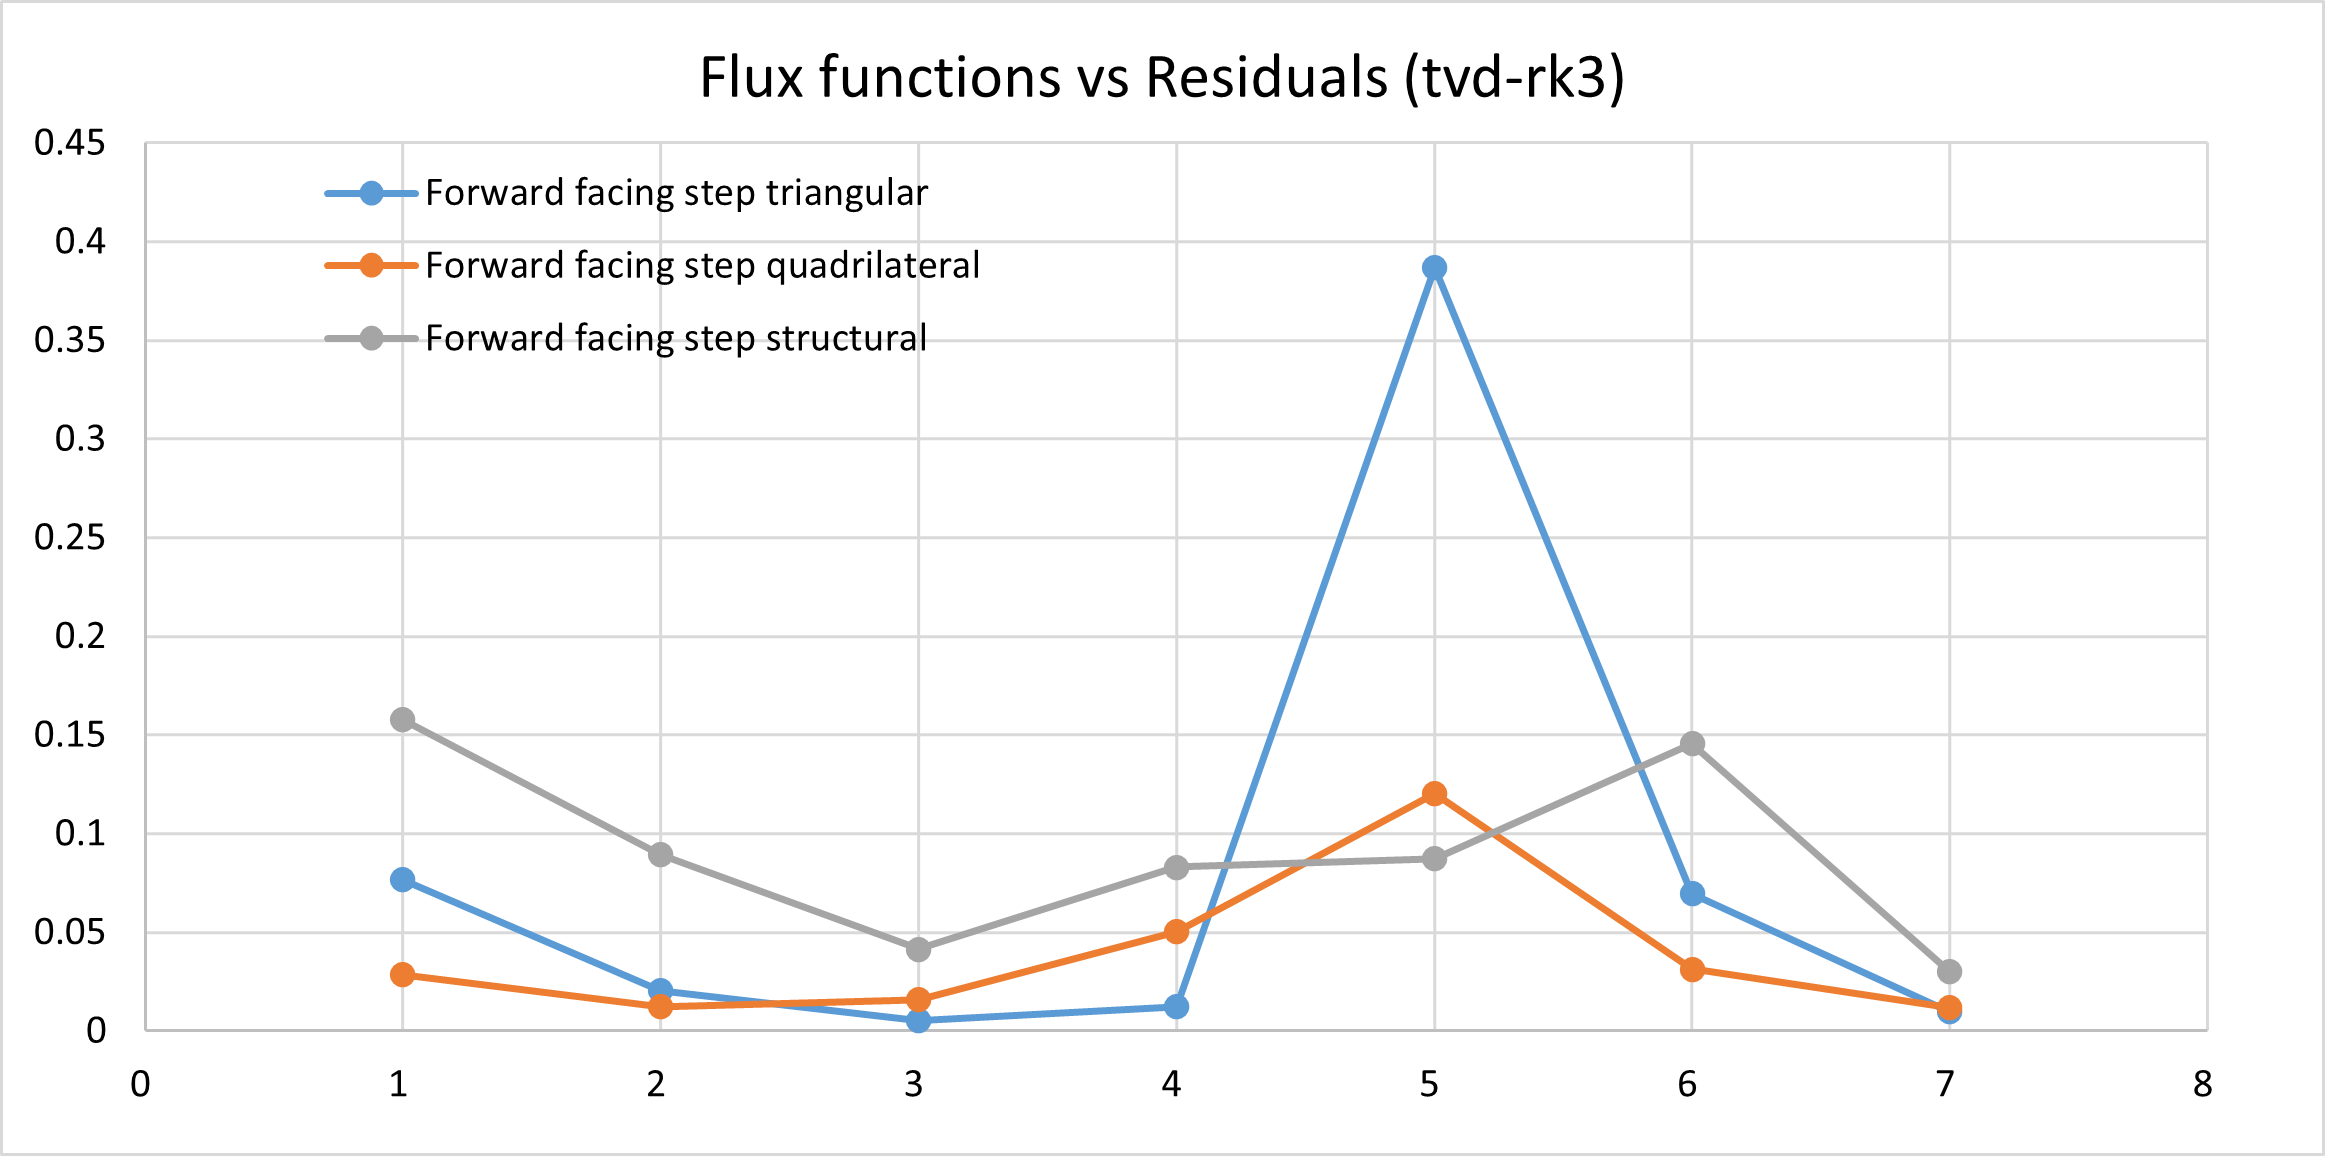
\includegraphics[width=0.75\linewidth]{HW4/tvd-rk3 Forward Facing.png}
    \caption{Forward Facing Step tvd-rk3}
\end{figure}

Starting with the first test case, the Forward Facing Step test case, as it can be seen clearly from Figures 13 and 14 the worst method for sharp bumps is $\text{AUSM}^+\text{-up}$ since it resulted in the biggest residual. However, this large residual is found when an unstructured mesh is used. For the structured case, the aforementioned method and test geometry resulted in a somewhat lower residual compared to the other methods. \\\par
An interesting observation is that although having the largest residual for one method, triangular mesh resulted in the lowest residuals for most of the methods tested except test cases 5 and 6. On the other hand, structured mesh geometry resulted in larger residuals for the most of test cases and the lowest for one test case which was $\text{AUSM}^+\text{-up}$. \\\par
Test case 6, HLLEM, resulted in the lowest residual when an unstructured quadrilateral test mesh was used which makes it worth commenting on since most cases were dominated by triangular mesh geometries.\\\par
Comparing time discretization methods is not an easy task since there are no distinct trends present. However one can easily compare two methods by using the tables shared (Table 7-Table 10). For triangular mesh, tvd-rk3 has the lower residual until $\text{AUSM}^+\text{-up}$. From this method and on lu-sgs is better. For quadrilateral test mesh the order changes. First lu-sgs has lower resudials until $\text{AUSM}^+\text{-up}$ then the other way around. For structured test case, lu-sgs has the lower residual for all cases.\\\par
Lastly comparing test methods is another subject to dive in. Back to the figures one can see a decreasing trend for triangular and structured until test method 3, Rotated-RoeM followed by an increase at method 4, AUSMPW+. Then their story diverges triangular one continues to rise while the structured one decreases. From here while the structured one increases, triangular one decreases. Lastly, they both decrease towards the method 8, Rusanov. Quadrilateral one increases up to case 5 and decreases from there.

\begin{figure}[H]
    \centering
    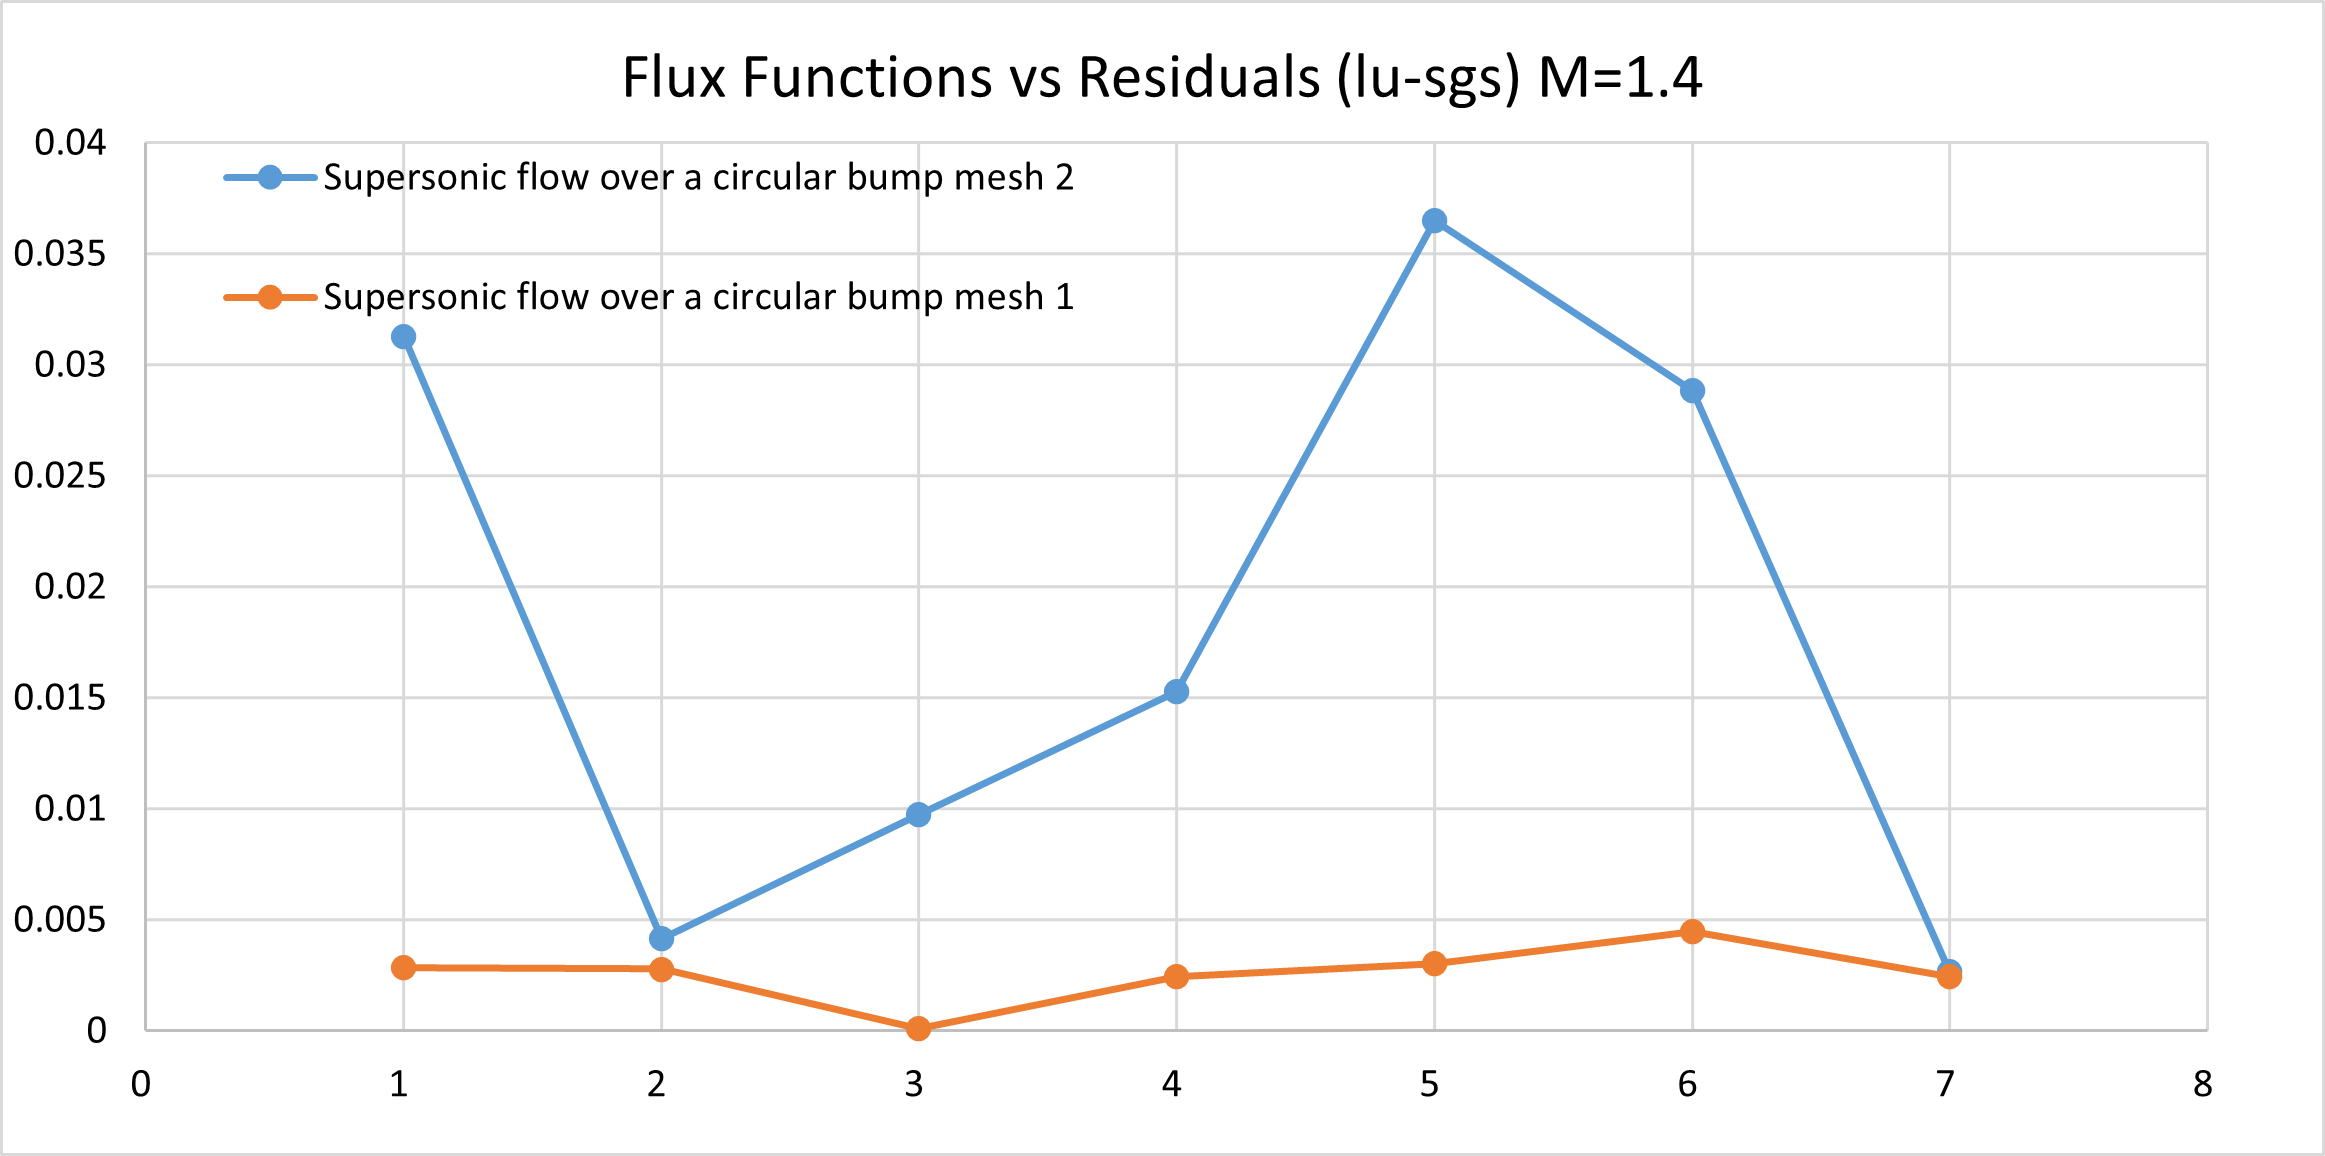
\includegraphics[width=0.75\linewidth]{HW4/Lu-sgs Circular 1.4.png}
    \caption{Supersonic Flow Over a Circular Bump lu-sgs}
\end{figure}
\begin{figure}[H]
    \centering
    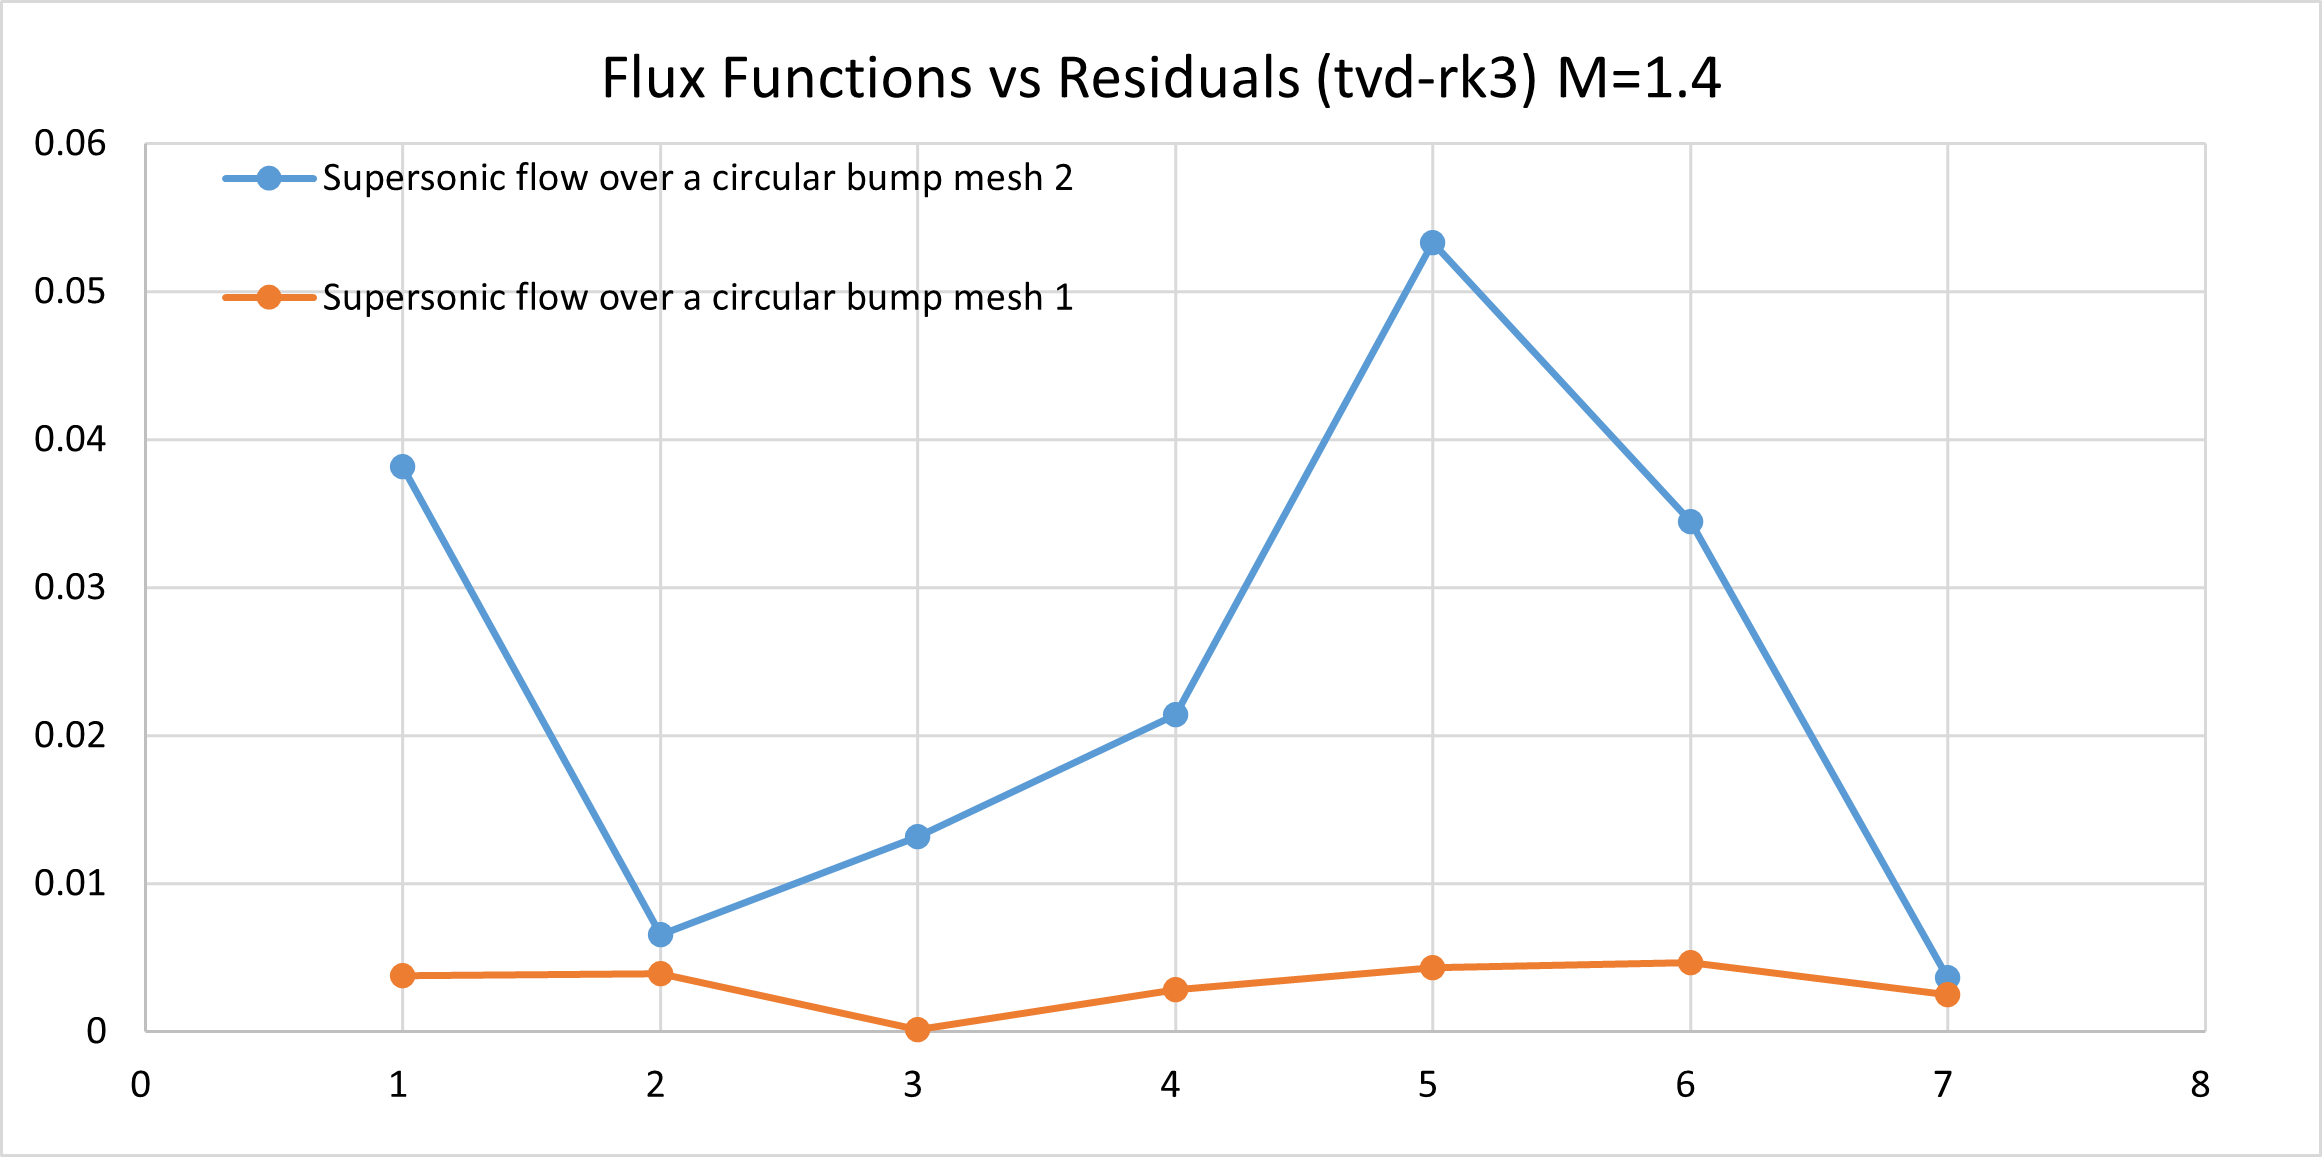
\includegraphics[width=0.75\linewidth]{HW4/tvd-rk3 Circular 1.4.png}
    \caption{Supersonic Flow Over a Circular Bump tvd-rk3}
\end{figure}
Continuing with Supersonic Flow Over a Circular Bump, one can observe that the quadrilateral mesh type results in a lower residual for all seven methods and time discretization methods. Only in lu-sgs discretization with method 7, Rusanov it results in a lower residual.\\\par

A general rule can be the independence of quadrilateral mesh type with lu-sgs discretization. Although methods change, this mesh resulted in a near-constant, low residual despite the triangular one being much finer than the quadrilateral one. It would not be wrong to say that for a circular obstacle in a supersonic flow, the suitable mesh is the quadrilateral one. Triangular one first drops down rapidly, and increases until test case 5, $\text{AUSM}^+\text{-up}$ is reached. From 5 and on it decreases once again. This last comment is observed for both time discretization methods.\\\par

Another observation is that the lowest residual is reached when the Rusanov method is used for the triangular test case, on the other hand for the first time a solution is converged. When Rotated-RoeM is used for quadrilateral mesh type, the residuals sunk below the convergence criteria.\\\par 
Also overall lu-sgs discretization resulted in lower residuals when compared to its counterpart.

\begin{figure}[H]
    \centering
    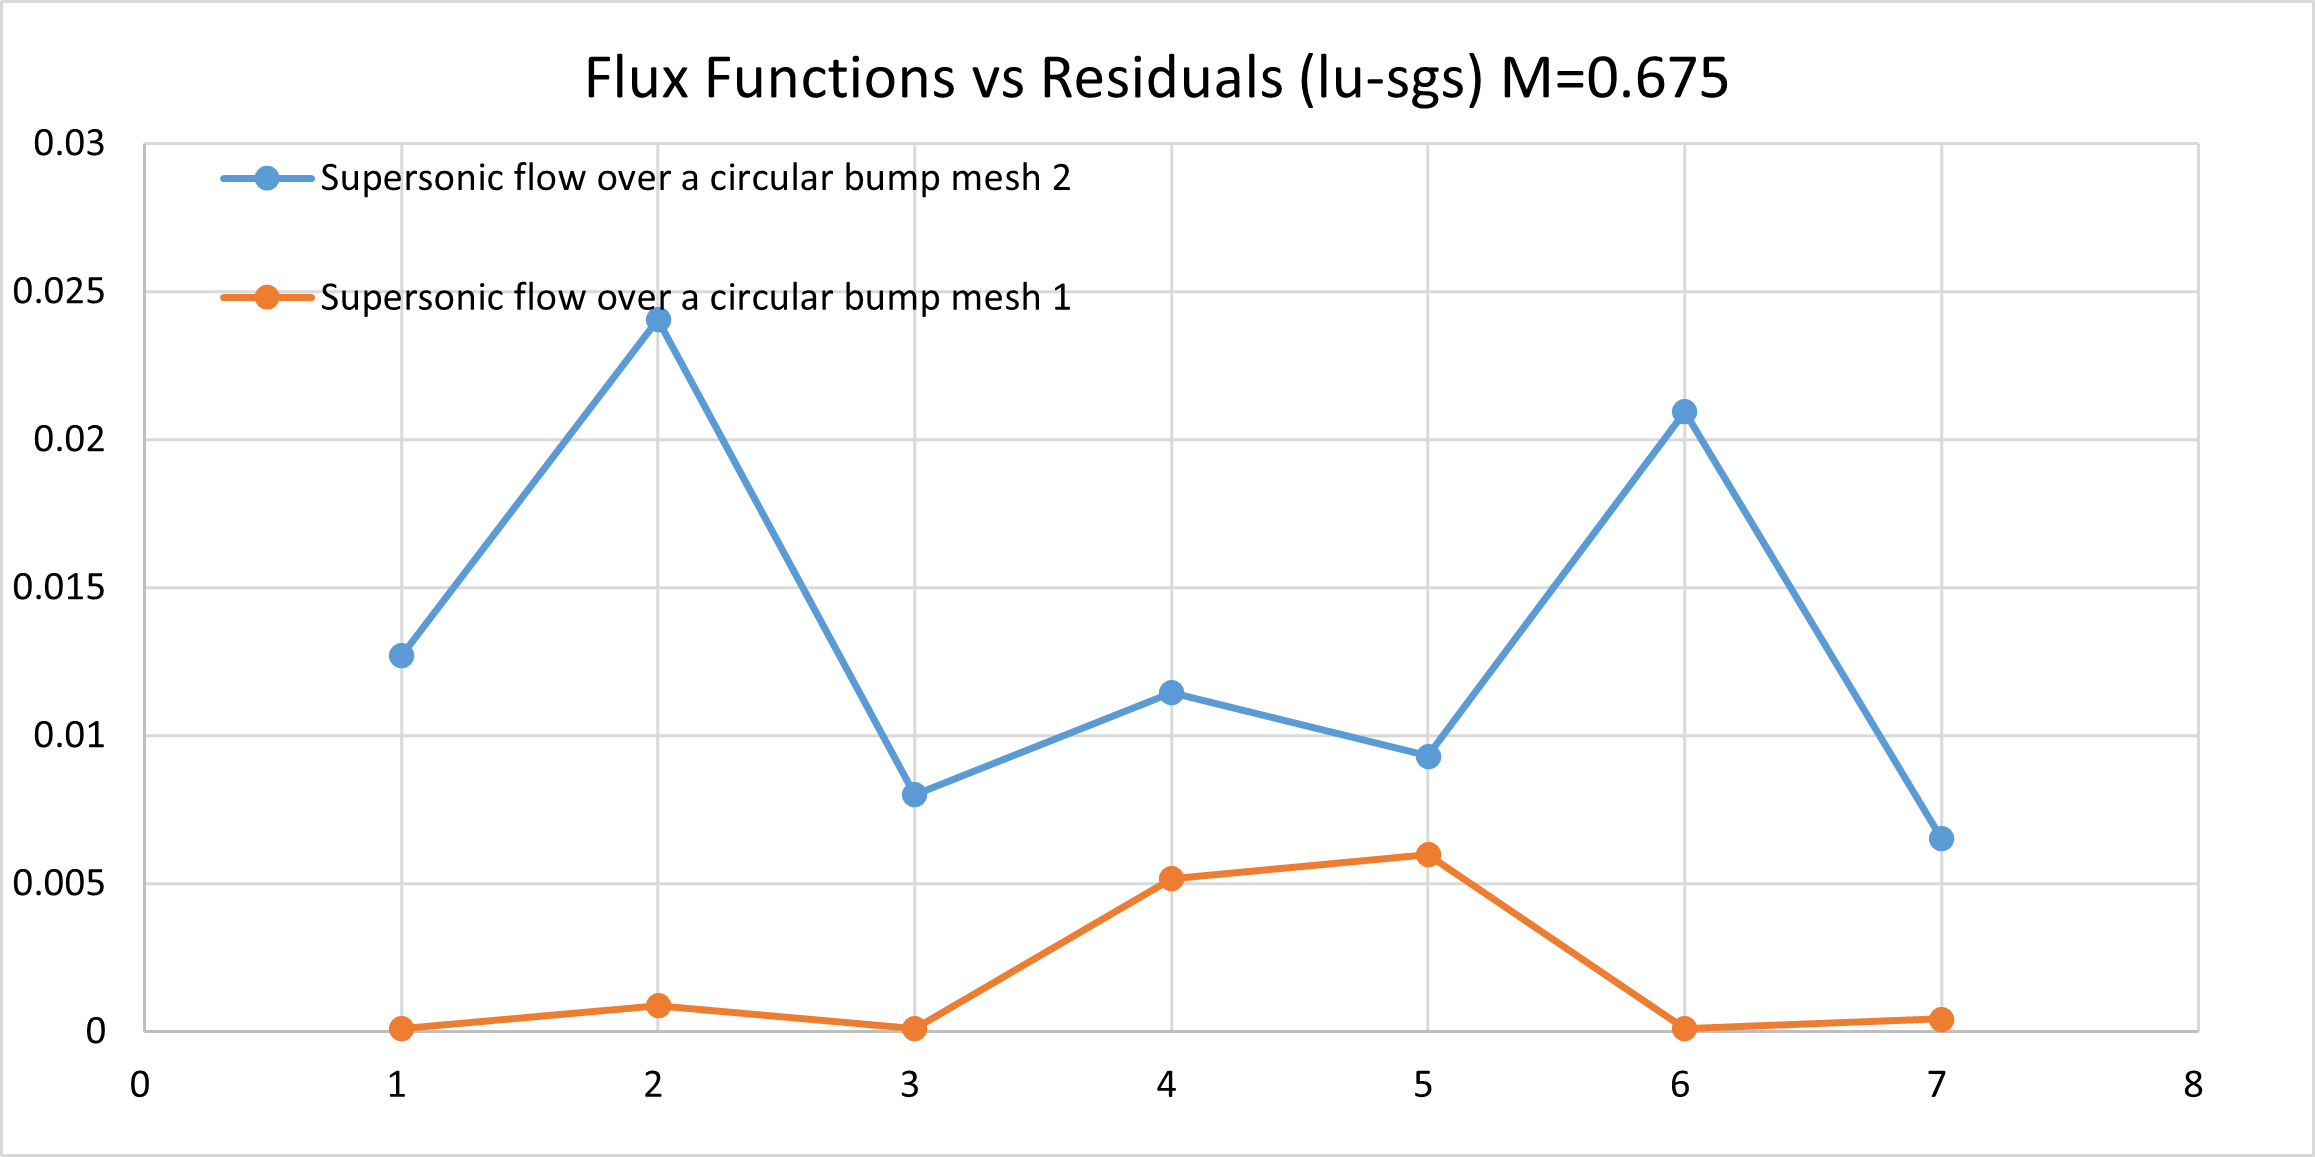
\includegraphics[width=0.75\linewidth]{HW4/Lu-sgs Circular M=0.675.png}
    \caption{Transonic Flow Over a Circular Bump lu-sgs}
\end{figure}
\begin{figure}[H]
    \centering
    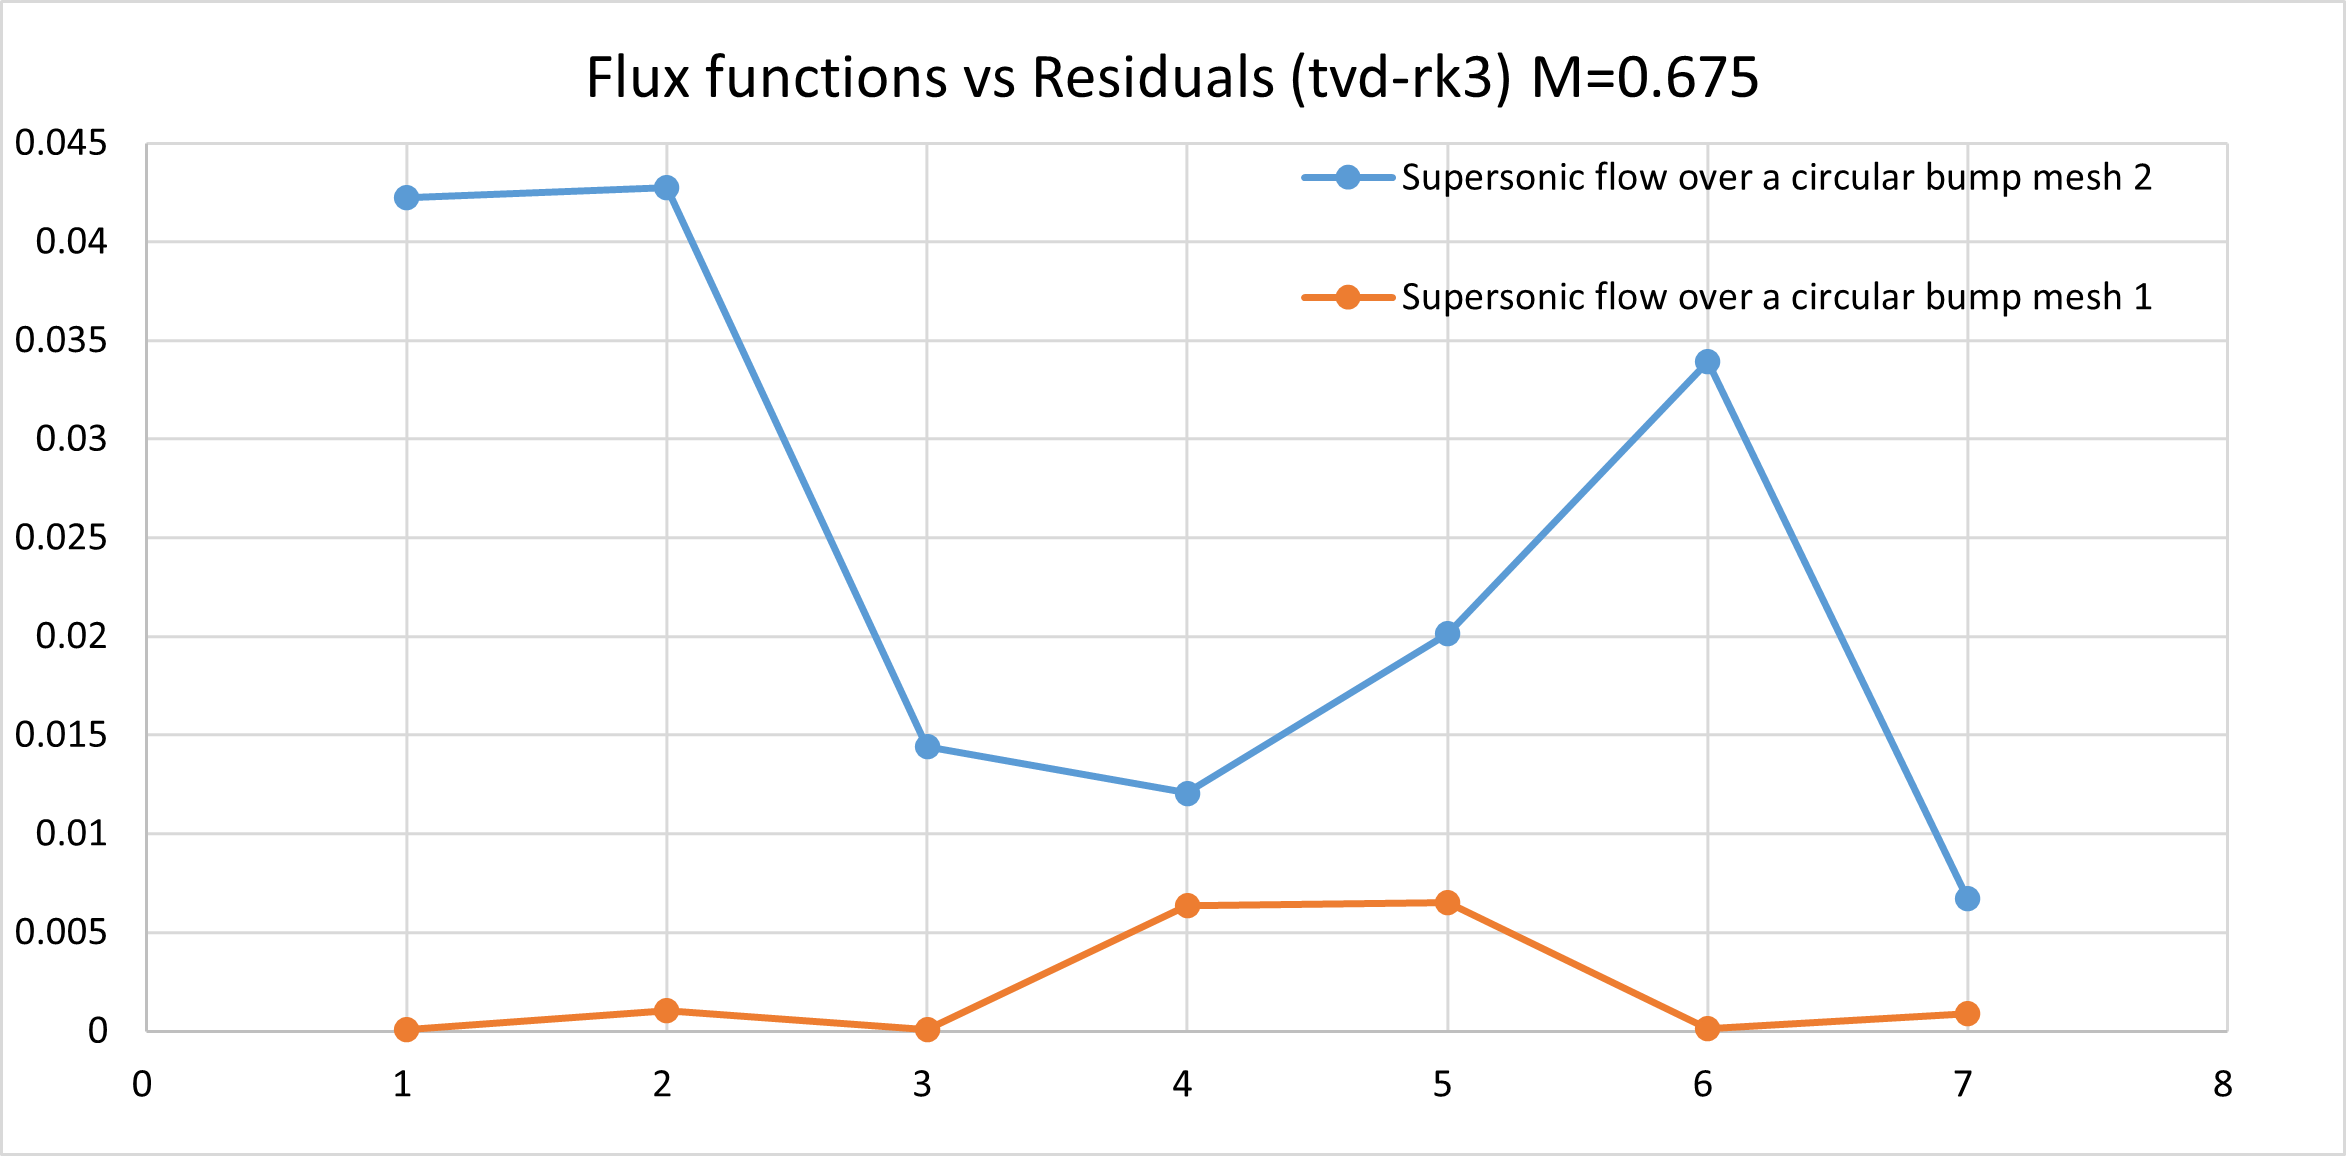
\includegraphics[width=0.75\linewidth]{HW4/tvd-rk3 Circular 0.675.png}
    \caption{Transonic Flow Over a Circular Bump tvd-rk3}
\end{figure}
Moving on to the Transonic Flow over a Circular Bump, the results are nothing similar to the previous case. Residuals increase and decrease regularly in the triangular mesh type and it is relatively high when compared to quadrilateral mesh type. This quadrilateral mesh type also fluctuates but is not as aggressive as the triangular mesh type. Despite pushing the boundaries of flux methods, this particular test case has the highest convergence rate up until now. It converges for Roe and Rotated-RoeM in both time discretization methods and HLLEM for lu-sgs discretization.\\\par
For the triangular mesh type lowest residual is reached when Rotated-RoeM is used, this is true for the quadrilateral mesh type since it converges when that method is used.\\\par
Also, one little observation is that lu-sgs discretized triangular mesh resembles the ears of a cat.

\begin{figure}[H]
    \centering
    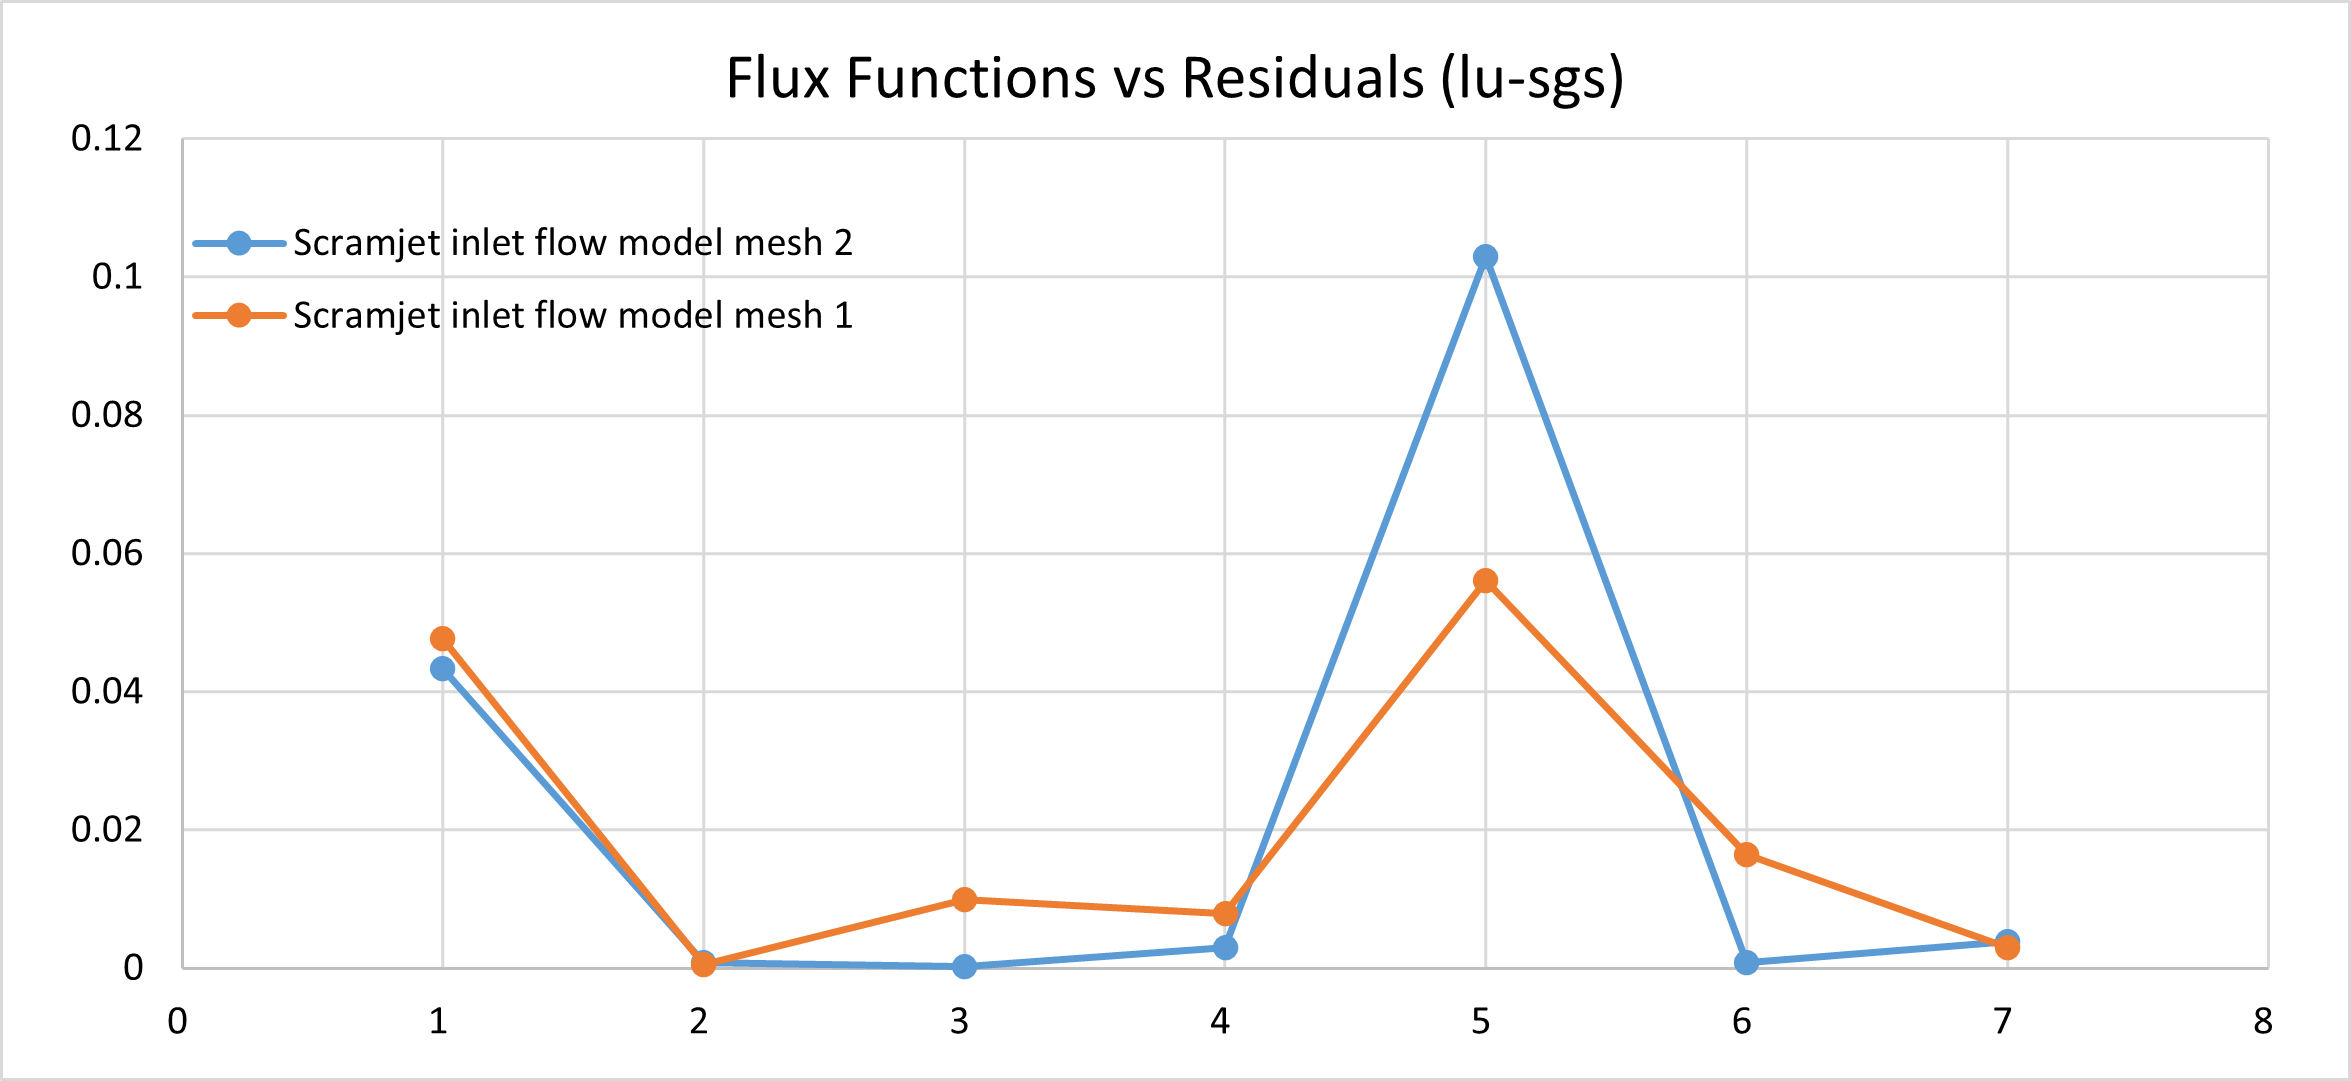
\includegraphics[width=0.75\linewidth]{HW4/Lu-sgs Scramjet.png}
    \caption{Scramjet Inlet Flow Model lu-sgs}
\end{figure}
\begin{figure}[H]
    \centering
    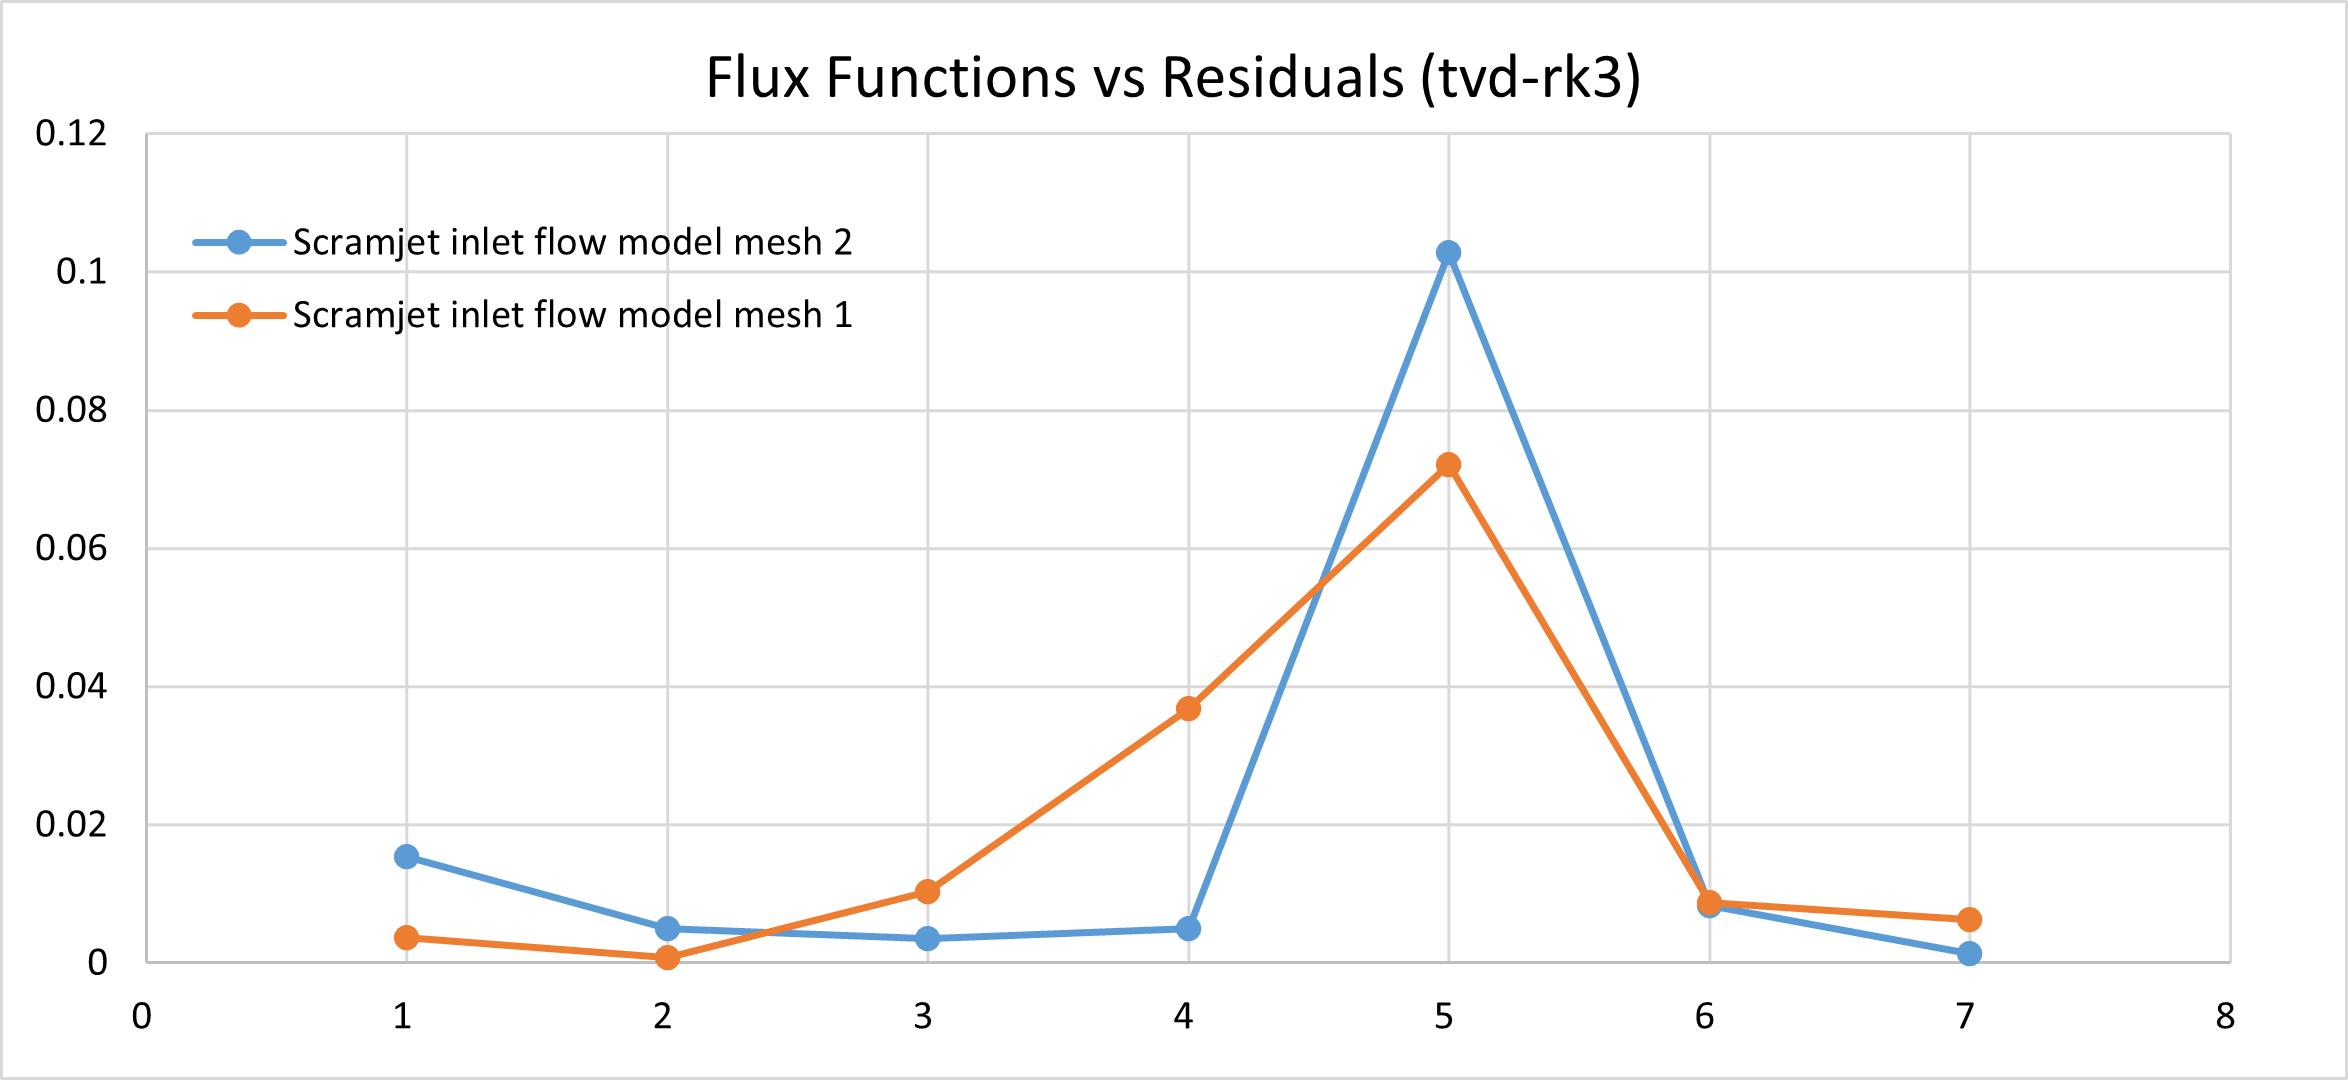
\includegraphics[width=0.75\linewidth]{HW4/tvd-rk3 Scramjet.png}
    \caption{Scramjet Inlet Flow Model tvd-rk3}
\end{figure}
Lastly, an intriguing flow problem of the inlet of a scram jet is investigated. Taking a quick gaze at Figure 21, one can see that mesh structures follow a similar pattern. They both start with a relatively high residual which is followed by a sharp descent. Then they both increase moderately until method 5, $\text{AUSM}^+\text{-up}$. When it reaches an abrupt jump happens then it is followed by a sharp decrease and another soft decrease follows the first one. About Figure 22 one can see that it has a similar trend with different initial conditions.\\\par
The discretization method of tvd-rk3 starts with surprisingly low residuals for both mesh types. While the mesh 2 has an increasing trend, the mesh1 counterpart decreases further. Overall mesh 1 has better results except when method 5, $\text{AUSM}^+\text{-up}$ in both and Rusonov in lu-sgs discretization is used.\\\par
The explicit method of discretization, tvd-rk3 resulted better only for the first two methods, the rest has a lower residual when tvd-rk3 method is used. \\\par

Comparison of the visualisation of these benchmarks with the literature is provided at the appendix

\appendix
\section{Comparison With Literature}
\subsection{Forward Facing Step Benchmark}
\begin{figure}[H]
    \centering
    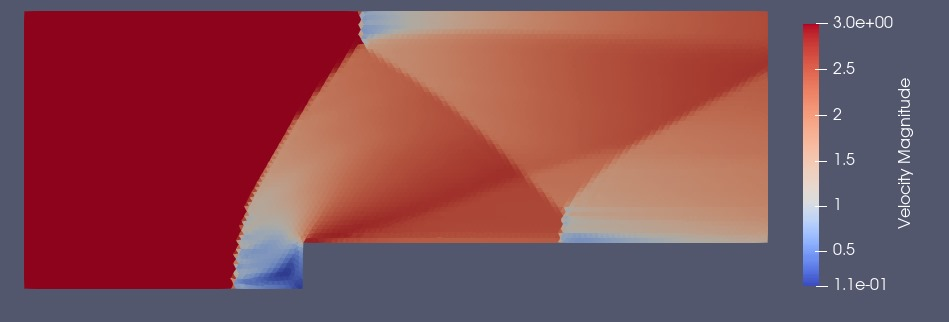
\includegraphics[width=0.8\linewidth]{HW4/Forward Facing Step.jpg}
    \caption{Visualization of the Forward Facing Step Benchmark (AUSMPW+ and lu-sgs)}
\end{figure}
\begin{figure}[H]
    \centering
    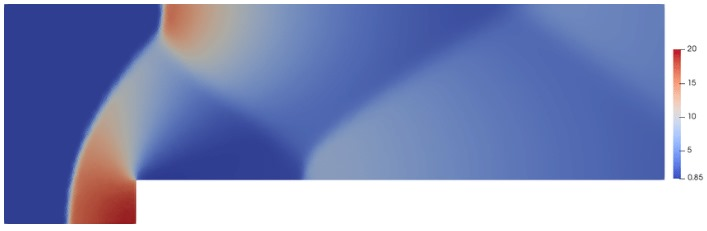
\includegraphics[width=0.8\linewidth]{HW4/ffs.jpeg}
    \caption{Forward Facing Step Benchmark from Literature (\cite{ffs})}
\end{figure} \par
As one can see, the visualization of the Forward Facing Step Benchmark obtained through \textit{ParaView} shows similarity with the results of \cite{ffs}
\newpage
\subsection{Supersonic Flow Over Circular Bump Benchmark}
\begin{figure}[H]
    \centering
    \includegraphics[width=0.8\linewidth]{HW4/supersonic flow over circular bump.jpg}
    \caption{Visualization of the Supersonic Flow Over Circular Bump Benchmark (AUSMPW+ and lu-sgs)}
\end{figure}
\begin{figure}[H]
    \centering
    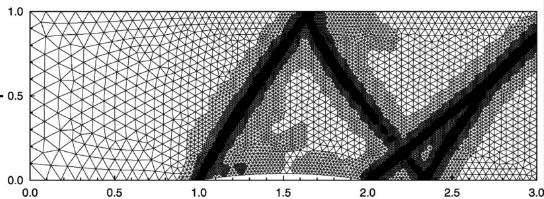
\includegraphics[width=1\linewidth]{HW4/sscb.jpeg}
    \caption{Supersonic Flow Over Circular Bump Benchmark from Literature (\cite{mach14})}
\end{figure} \par
Similarly, the obtained visualization shows similarity with the literature for the Supersonic Flow Over Circular Bump Benchmark (\cite{mach14})
\newpage
\subsection{Transonic Flow Over Circular Bump}
\begin{figure}[H]
    \centering
    \includegraphics[width=0.8\linewidth]{HW4/Transonic flow over circular bump.jpg}
    \caption{Visualization of the Transonic Flow Over Circular Bump Benchmark (AUSMPW+ and lu-sgs)}
\end{figure}
\begin{figure}[H]
    \centering
    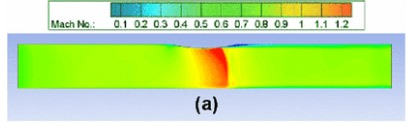
\includegraphics[width=0.8\linewidth]{HW4/ts.jpeg}
    \caption{Transonic Flow Over Circular Bump Benchmark from Literature (\cite{cs})}
\end{figure}
Unsurprisingly \mefvm produces the desired result.
\newpage
\subsection{Scramjet Inlet Flow Model Benchmark}
\begin{figure}[H]
    \centering
    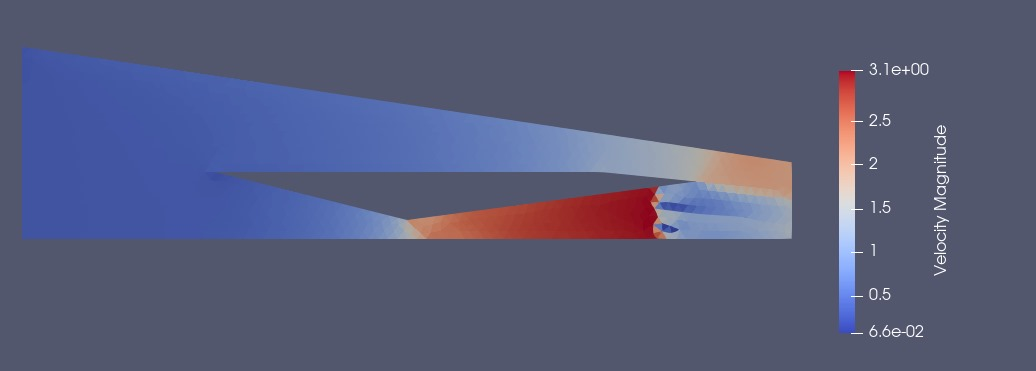
\includegraphics[width=0.8\linewidth]{HW4/scrambiz.jpeg}
    \caption{Visualization of the Scramjet Inlet Flow Model Benchmark (AUSMPW+ and lu-sgs)}
\end{figure}
\begin{figure}[H]
    \centering
    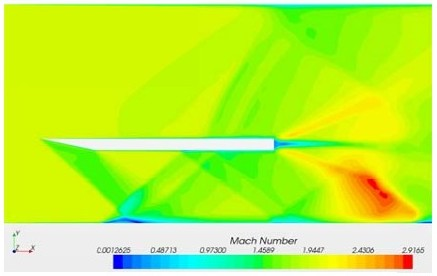
\includegraphics[width=0.8\linewidth]{HW4/scram.jpeg}
    \caption{Scramjet Inlet Flow Model Benchmark from Literature (\cite{scram})}
\end{figure}
As one can see, the figures are not similar. This is due to the fact that with the given case, a normal shockwave stands at the entrance of the model causing the actual Mach number of the inlet condition to be around 0.5. If the inlet Mach number is increased to 3.2 the following visualization is obtained with \mefvm.
\begin{figure}[H]
    \centering
    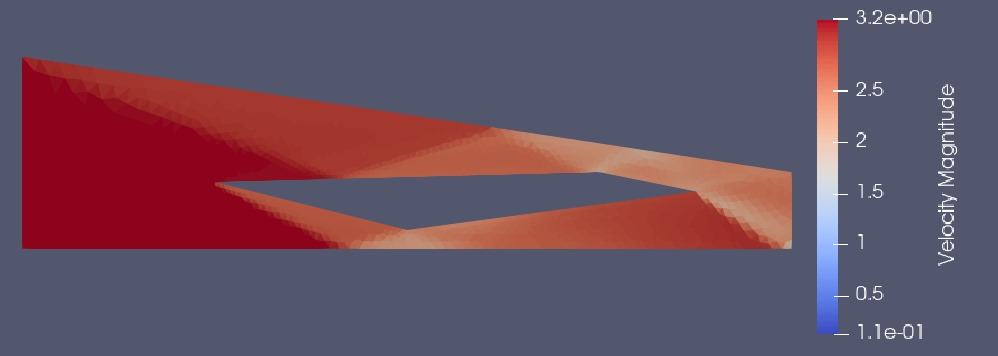
\includegraphics[width=0.8\linewidth]{HW4/m3.2scram.jpeg}
    \caption{Visualization of the Scramjet Inlet Flow Model Benchmark Adjusted with M = 3.2 for Inlet Case (AUSMPW+ and lu-sgs)}
\end{figure}
The output shows a resemblance to the literature showing the oblique shock waves desirable in scramjet applications.
\newpage
\printbibliography
\end{document}